%\title{Phi Sigma Symposium Presentation}
\documentclass[10pt]{beamer}

\usetheme[progressbar=frametitle]{metropolis}
\usepackage{appendixnumberbeamer}

\usepackage{booktabs}
\usepackage[scale=2]{ccicons}

\usepackage{pgfplots}
\usepgfplotslibrary{dateplot}

\usepackage{xspace}
\usepackage{mathtools}
\usepackage{bm}
\usepackage[export]{adjustbox}

\usepackage{graphicx}
\usepackage{sidecap}
\sidecaptionvpos{figure}{c}
\usepackage{hyperref}
\usepackage{tikz}
\usepackage{multimedia}
\usepackage{media9}

\usepackage{array}
\usepackage{multirow}
\usepackage{setspace}

\DeclarePairedDelimiter\abs{\lvert}{\rvert}%
\DeclarePairedDelimiter\norm{\lVert}{\rVert}%
\newcommand{\themename}{\textbf{\textsc{metropolis}}\xspace}

\title{Modeling the Collective \\ Behavior of Ants on Uneven Terrain}
\subtitle{Phi Sigma Undergraduate Research Symposium}
\date{April 1st, 2017}
\author{Matthew Moreno$^{1}$, Dr. Jason Graham$^{2}$, Dr. Simon Garnier$^{3}$} % Author(s)

\institute{$^{1}$University of Puget Sound \\ [0.5ex]
		   $^{2}$University of Scranton \\ [0.5ex]
           $^{3}$New Jersey Institute of Technology }

\titlegraphic{\hfill
\includegraphics[height=1.5cm]{images/mbiwtext}}

\begin{document}

\maketitle

% \begin{frame}{Overview}
%   \setbeamertemplate{section in toc}[sections numbered]
%   \tableofcontents
% \end{frame}

\section{Introduction}

\begin{subsection}{Motivation}
\begin{frame}{Motivation}

\vspace{1em}
\begin{figure}
\begin{columns}%
        \begin{column}{0.8\textwidth}%
            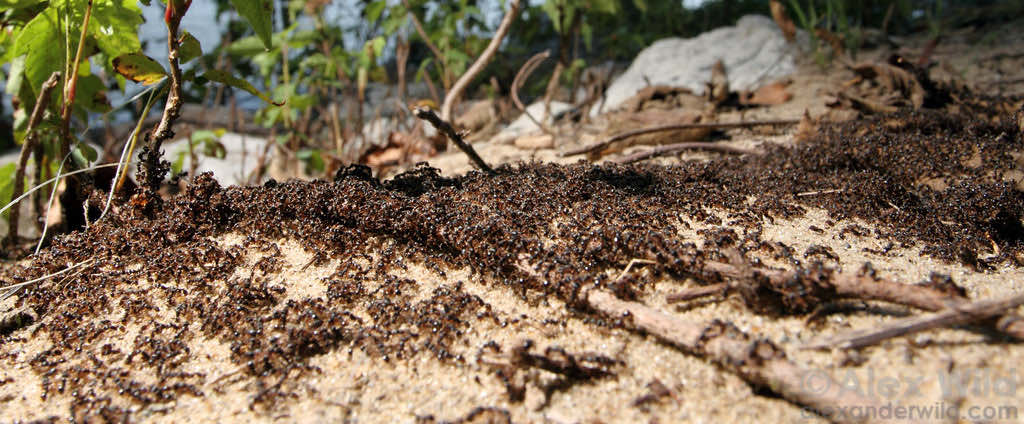
\includegraphics[width=\textwidth,right]{images/ant_battle1-XL_reduced}
        \end{column}%
        \begin{column}{0.2\textwidth}%
            \caption{Ant traffic \scriptsize{\cite{alexander_wild_ant_battle1-xl.jpg_????}}}
        \end{column}%
    \end{columns}
\end{figure}

\begin{figure}
\begin{columns}%
        \begin{column}{0.8\textwidth}%
            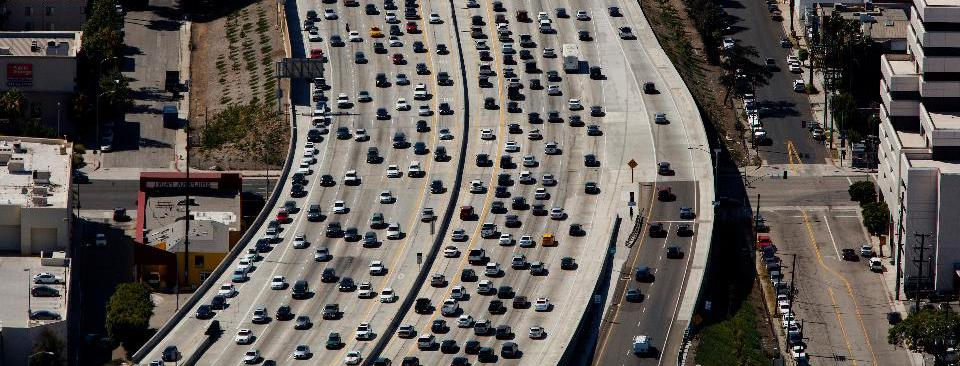
\includegraphics[width=\textwidth,right]{images/960x0_reduced}
        \end{column}%
        \begin{column}{0.2\textwidth}%
            \caption{Human traffic \scriptsize{\cite{patrick_t._fallon_960x0.jpg_2015}}}
        \end{column}%
    \end{columns}
\end{figure}

\end{frame}

\end{subsection}

\begin{subsection}{Background}

\begin{frame}{Background}
\begin{figure}
\begin{columns}%
        \begin{column}{0.8\textwidth}%
            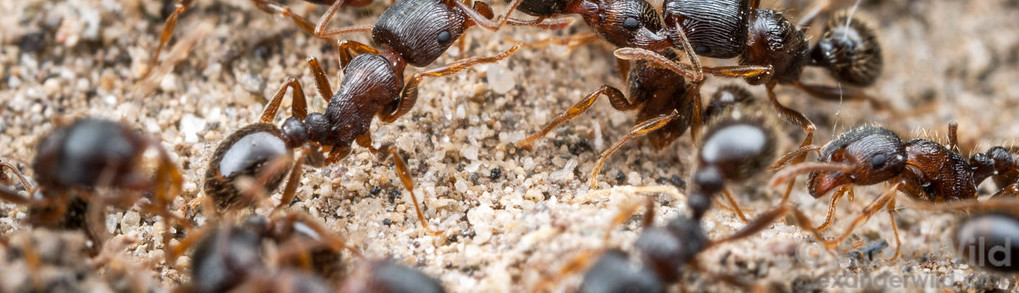
\includegraphics[width=\textwidth,right]{images/caespitum16j-XL}
        \end{column}%
        \begin{column}{0.2\textwidth}%
            \caption{\textit{Tetramorium caespitum} \scriptsize{\cite{alexander_wild_caespitum-16j-xl.jpg_????}}}
        \end{column}%
    \end{columns}
\end{figure}
The collective foraging behavior of ants is well studied, including
\begin{itemize}
	\item the strategies ants use to engage in foraging behavior {\scriptsize\cite{camazine_self-organization_2003}}
    \item how ants tend to select the shortest path to food {\scriptsize\cite{camazine_self-organization_2003}}
    \item how ants tend to select the richest food source {\scriptsize\cite{camazine_self-organization_2003}}
    \item approaches to mathematical modeling of ant foraging  {\scriptsize\cite{perna_individual_2012,ryan_model_2016}}
\end{itemize}

\end{frame}
\end{subsection}


\begin{subsection}{Research Question}

\begin{frame}{Research Question}
\begin{columns}[T,onlytextwidth]
\column{0.5\textwidth}
\begin{itemize}
	\item \textbf{How does terrain affect the foraging path chosen by ants?}
	\item To travel between nest to food, do ants tend to select
    	\begin{itemize}
        	\item the shortest path,
            \item the quickest path,
            %\item the most energy efficient path,
            \item some compromise between these, or
            \item some other path all together?
          \end{itemize}
    \item How might individual ant behaviors on uneven terrain contribute to collective decision making?
\end{itemize}
\column{0.1\textwidth}
\column{0.4\textwidth}
\begin{figure}
        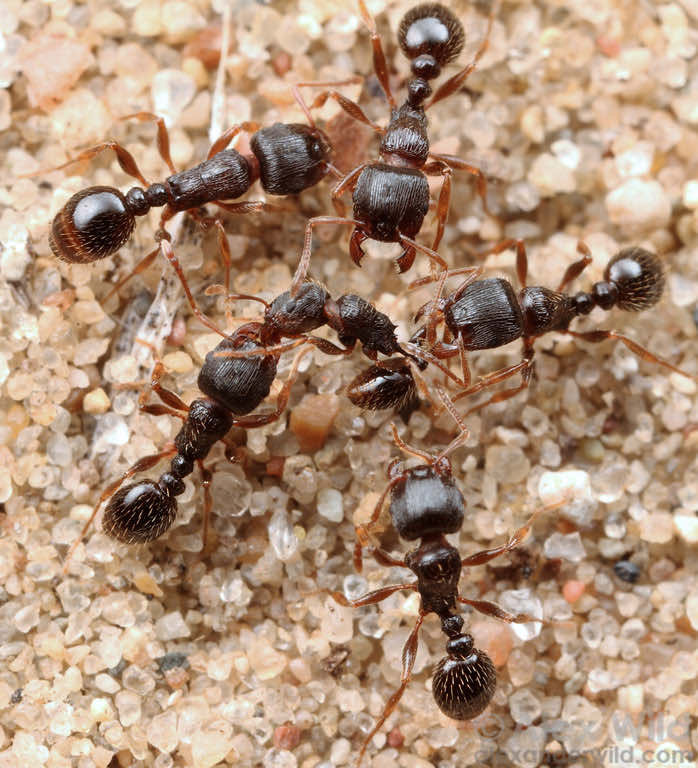
\includegraphics[width=\textwidth]{images/ant_battle2-XL_reduced}
        \caption{\textit{Tetramorium caespitum} \scriptsize{\cite{alexander_wild_ant_battle2-xl.jpg_????}}}
\end{figure}
\end{columns}
\end{frame}

\end{subsection}

\section{Approach}

\begin{subsection}{Experimental Design and Modeling Objectives}

\begin{frame}{Experimental Design}

\begin{figure}
    	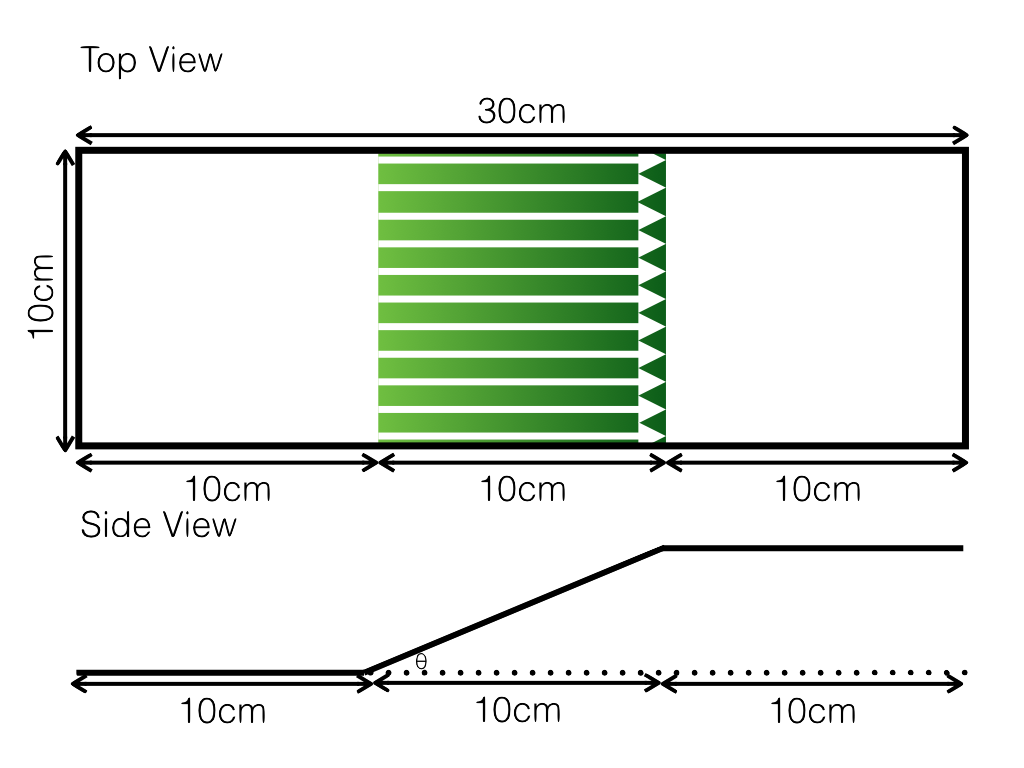
\includegraphics[width=0.8\textwidth]{images/model_components_cartoons_011}
      \caption{Arena terrain scheme}
 \end{figure}
\end{frame}

\begin{frame}{Modeling Objectives}
\vspace{-4ex}
\begin{figure}
\begin{tabular}{*{3}{>{\centering\arraybackslash}p{0.3\textwidth}}}
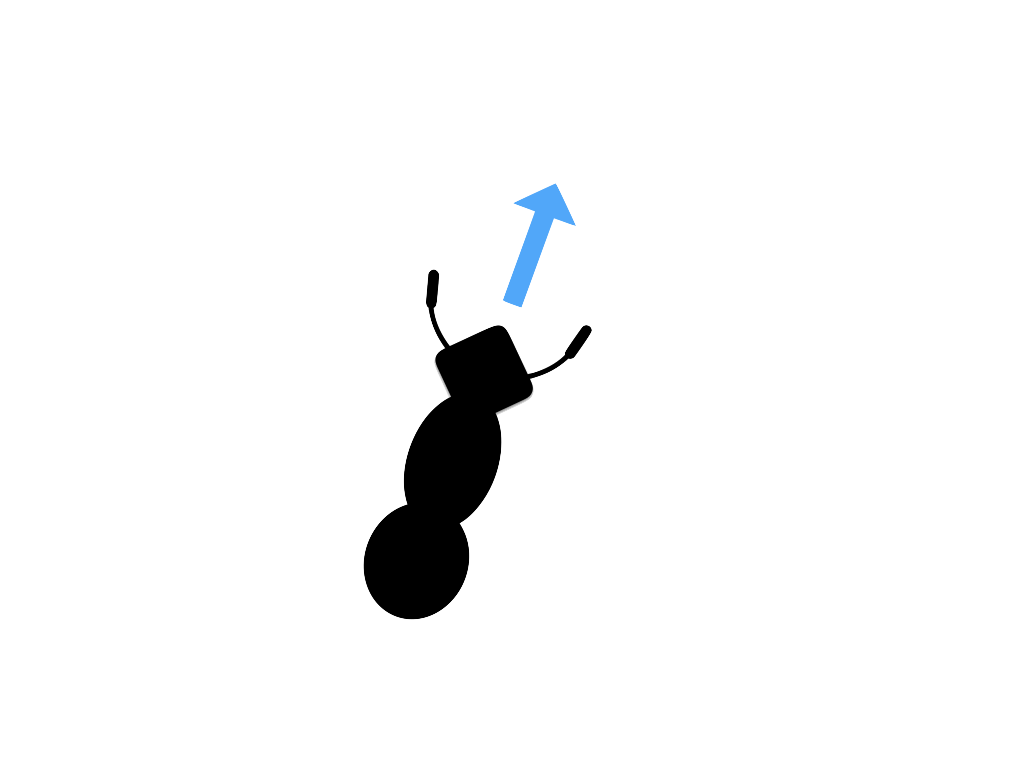
\includegraphics[width=0.20\textwidth]{images/model_components_cartoons_001} &
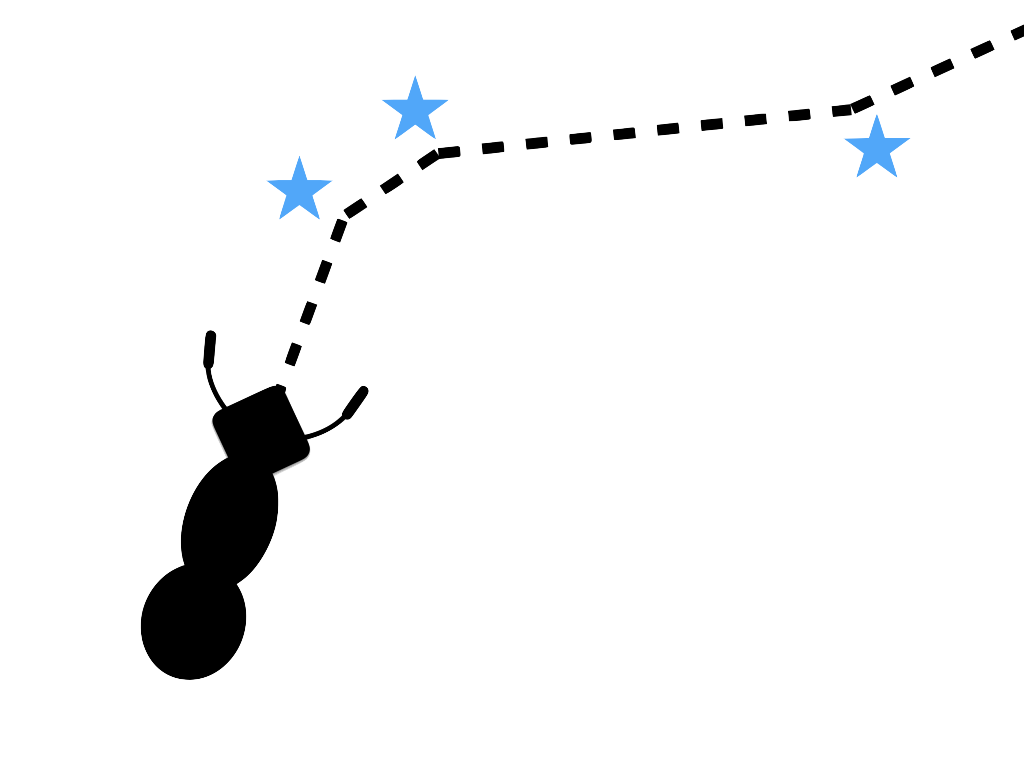
\includegraphics[width=0.20\textwidth]{images/model_components_cartoons_009} &
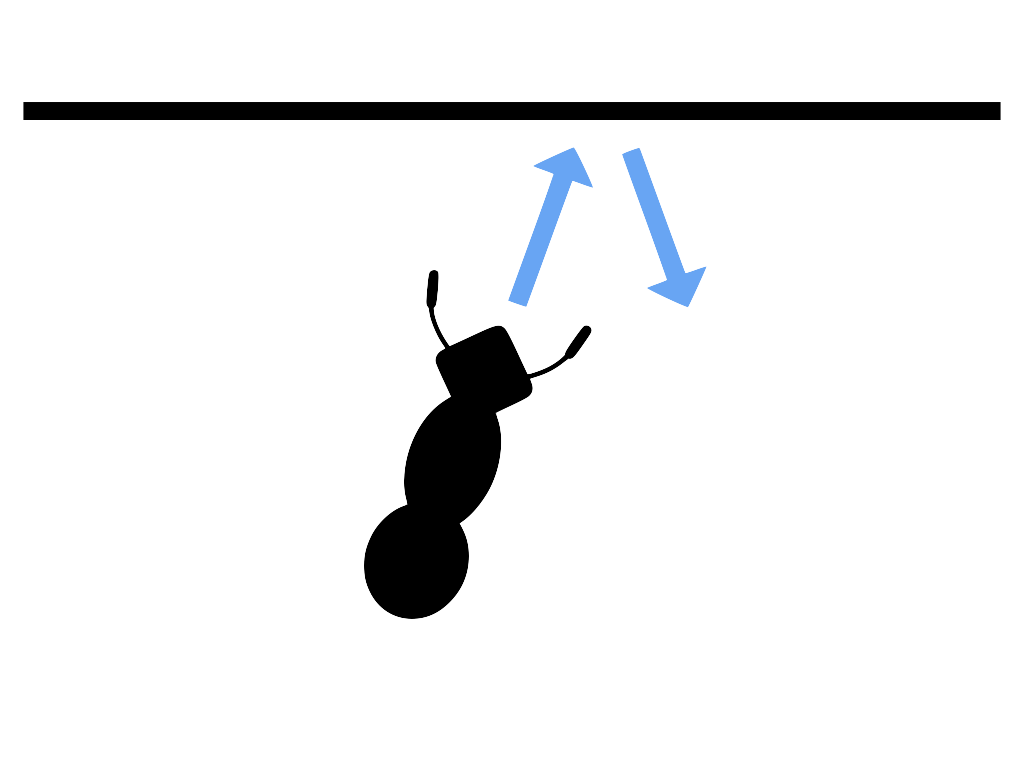
\includegraphics[width=0.20\textwidth]{images/model_components_cartoons_013} \\
\begin{spacing}{1.0}
{\footnotesize
Self Propulsion}
\end{spacing} &
\begin{spacing}{1.0}
{\footnotesize
Random Reorientation}
\end{spacing} &
\begin{spacing}{1.0}
{\footnotesize
Containment}
\end{spacing} 
\\[-0.75cm]
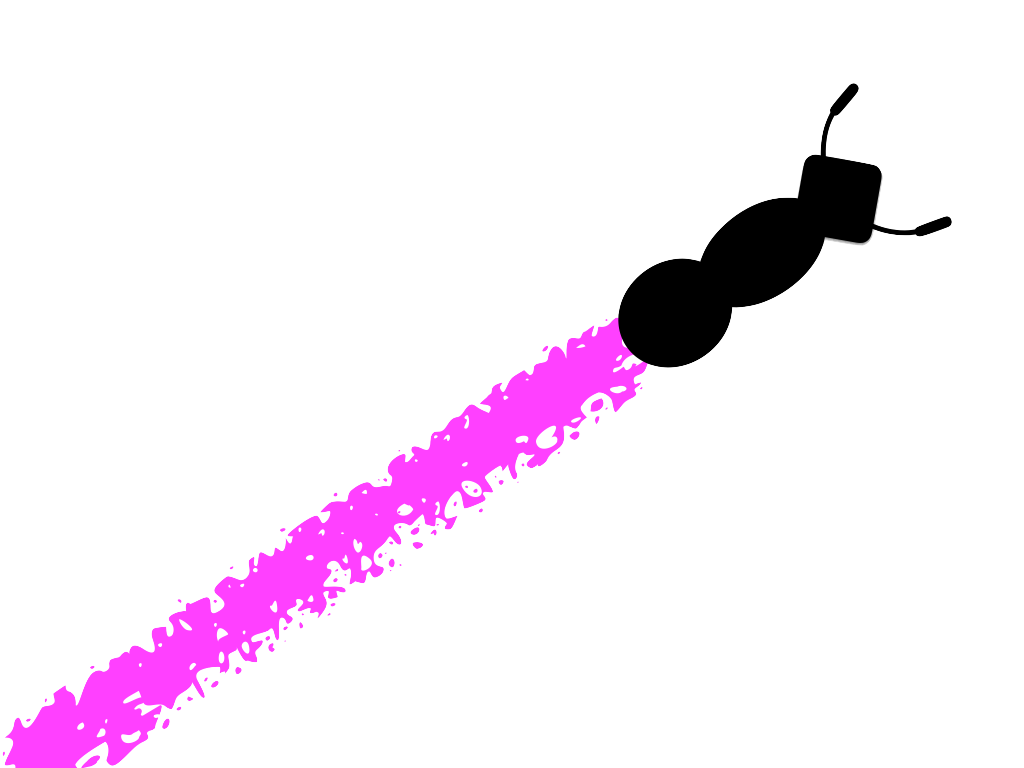
\includegraphics[width=0.20\textwidth]{images/model_components_cartoons_006} &

\includegraphics[width=0.20\textwidth]{images/model_components_cartoons_008} &
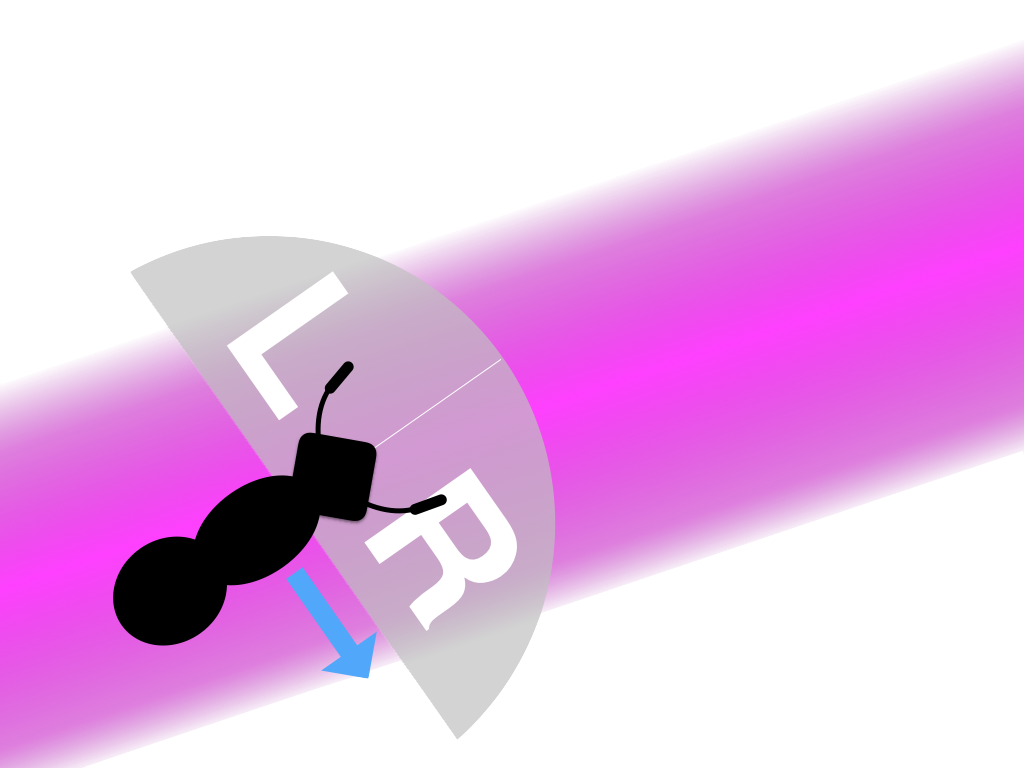
\includegraphics[width=0.20\textwidth]{images/model_components_cartoons_007} \\
\begin{spacing}{1.0}
\raggedright{\footnotesize
Pheromone Deposit}
\end{spacing} &
\begin{spacing}{1.0}
{\footnotesize
Pheromone Evaporation}
\end{spacing} &
\begin{spacing}{1.0}
{\footnotesize
Pheromone Response}
\end{spacing} \\[-0.75cm]
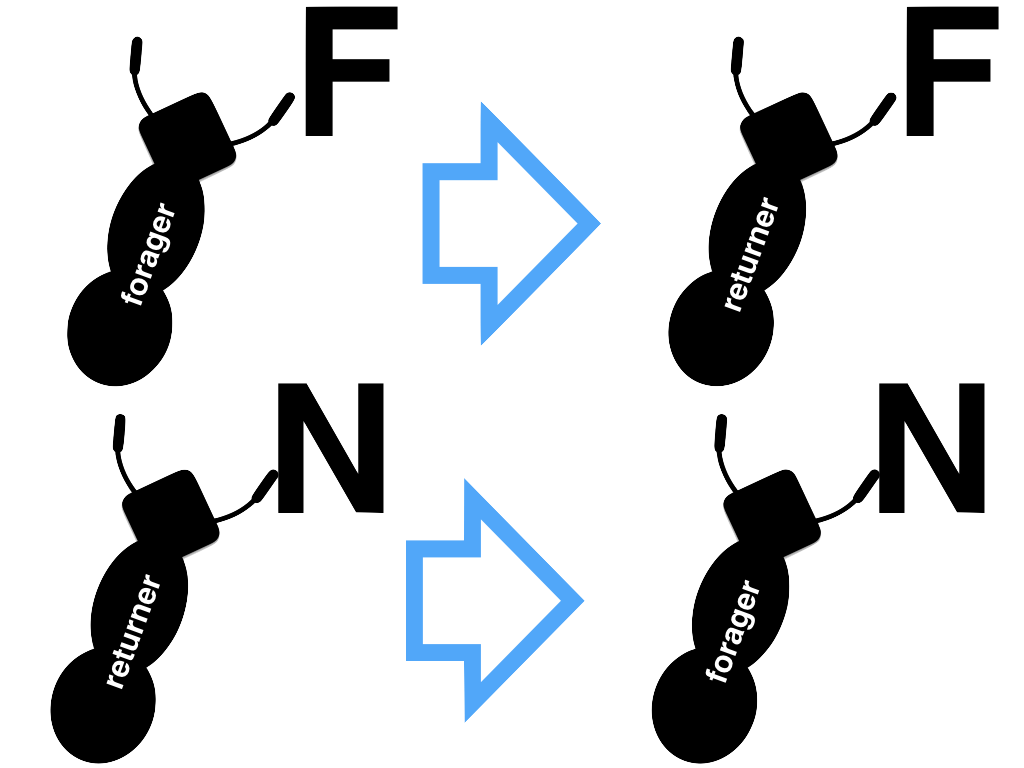
\includegraphics[width=0.20\textwidth]{images/model_components_cartoons_005} &
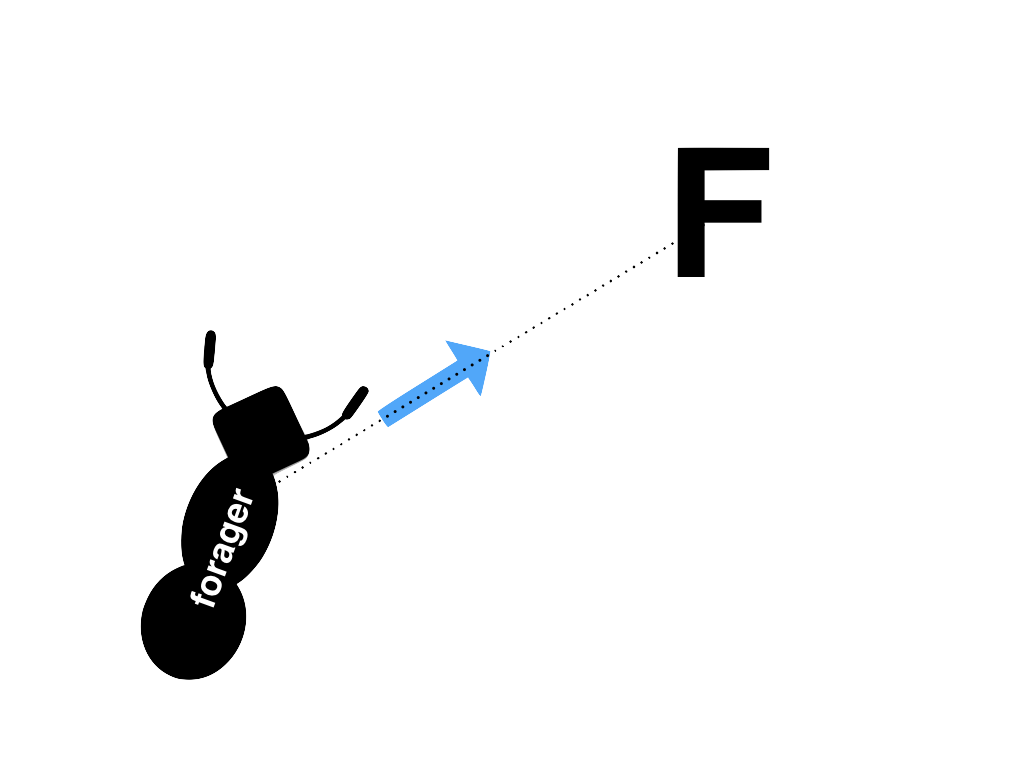
\includegraphics[width=0.20\textwidth]{images/model_components_cartoons_004} &
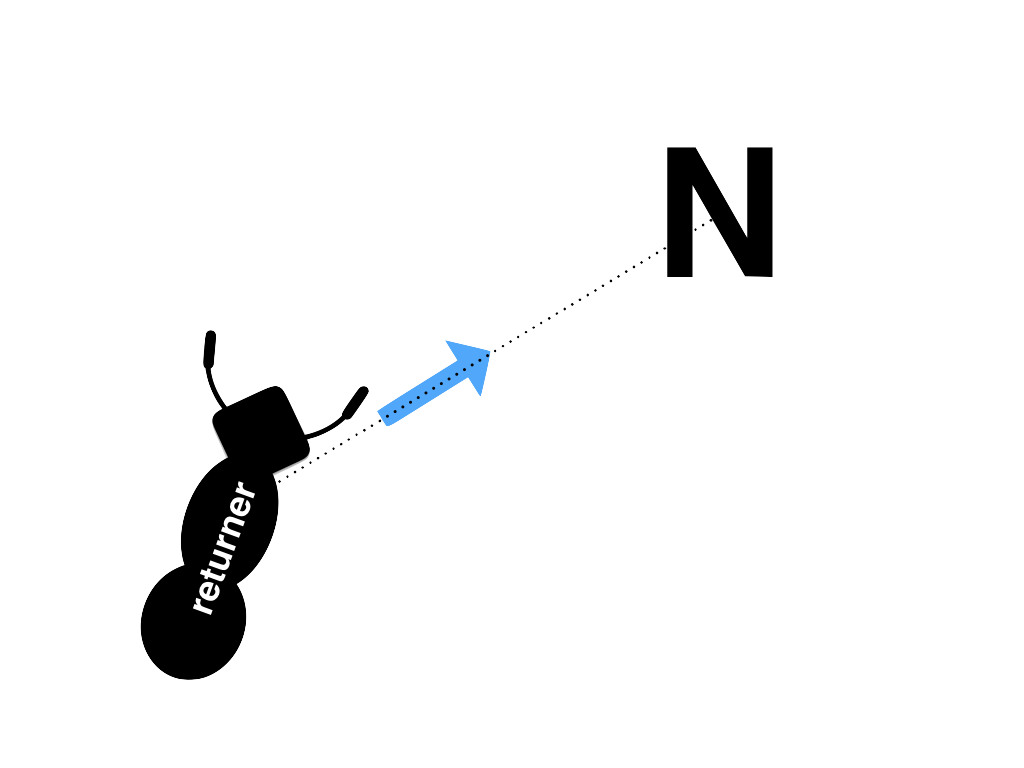
\includegraphics[width=0.20\textwidth]{images/model_components_cartoons_002} \\ 
\begin{spacing}{1.0}
\raggedright{\footnotesize
Forager/Returner Roles}
\end{spacing} &
\begin{spacing}{1.0}
{\footnotesize
Food Attraction}
\end{spacing} &
\begin{spacing}{1.0}
{\footnotesize
Nest Attraction}
\end{spacing} \\[-0.75cm]
\end{tabular}
\caption{Major modeling considerations}
\end{figure}
\end{frame}
\end{subsection}

\begin{subsection}{Events}
% \begin{frame}{Events}
% \begin{itemize}
% 	\item certain conditions trigger instantaneous changes in state variables
%     \item example: bouncing ball
% \end{itemize}
%   \begin{figure}
%   	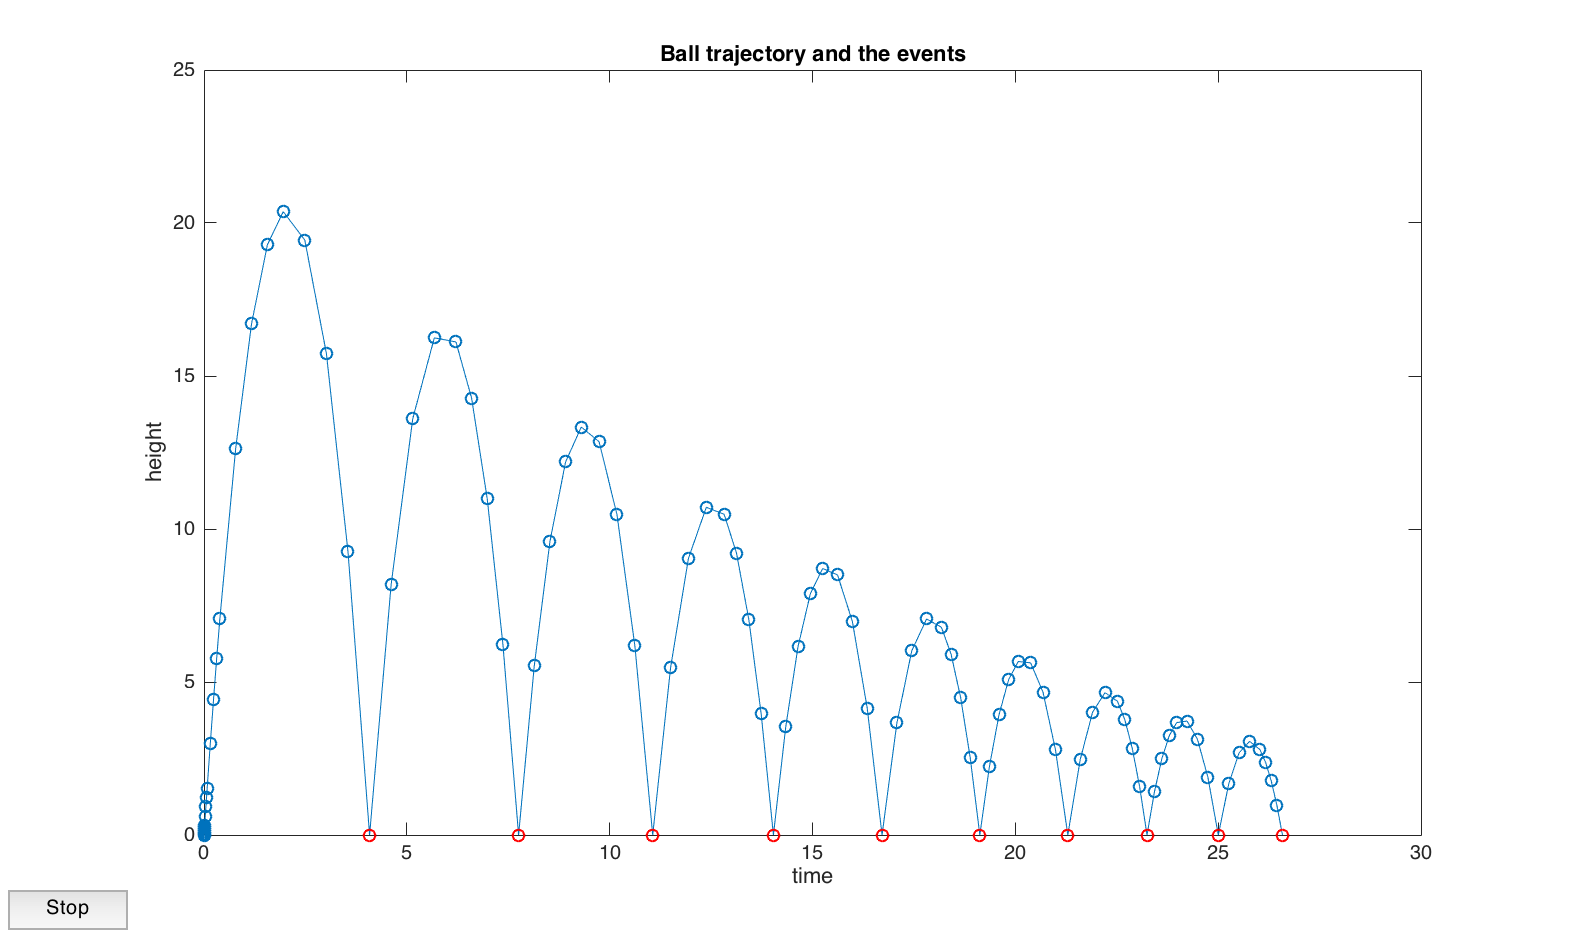
\includegraphics[height=5cm]{images/bouncing-ball}
%     \caption{Matlab ballode example}
%   \end{figure}
% \end{frame}

% \begin{frame}{Events}
% uses:
% \begin{itemize}
% 	\item ``bouncing'' ants off the arena walls
% 	\item switching between forager and returner roles
%   \item random reorientation events

% \end{itemize}
% \end{frame}

\begin{frame}{Random Reorientation Events \scriptsize{\cite{khuong_how_2013}}}
\begin{columns}[T,onlytextwidth]
\column{0.45\textwidth}
\begin{align*}
\frac{d}{dt} \begin{pmatrix}\vec{x}\\\vec{v}\\s\end{pmatrix} = \begin{pmatrix}\ldots \\ \ldots\\ \norm{v}\end{pmatrix}
\end{align*}
\column{0.1\textwidth}
\column{0.45\textwidth}
\begin{align*}
\theta_{\operatorname{new}} = \theta_{\operatorname{old}} + \bm{T} \\
s = 0 \\
s_{\operatorname{thresh}} = \bm{X}
\end{align*}
\end{columns}
\vspace{-2ex}
\begin{figure}
	\begin{columns}[T, onlytextwidth]
		\column{0.1\textwidth}
		\column{0.4\textwidth}
		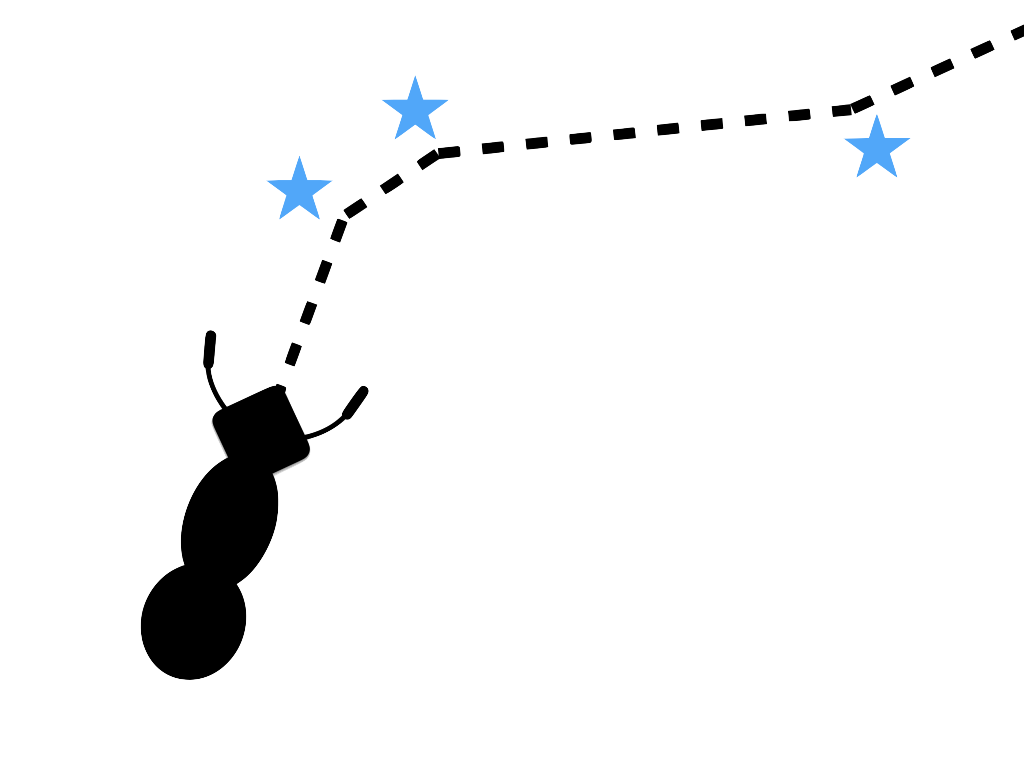
\includegraphics[width=\textwidth]{images/model_components_cartoons_009}
		\column{0.4\textwidth}
		\caption{\footnotesize{``Boltzmann walker'' cartoon; blue stars denote random reorientation events}}
		\column{0.1\textwidth}
	\end{columns}
\end{figure}
\vspace{-6ex}
\begin{itemize}
		%\item ant ``keeps track'' of how far it has traveled, $s$
    \item upon reaching a threshold distance ($s > s_{\operatorname{thresh}}$), the ant experiences a ``reorientation event''
    \item the threshold distance is generated from an exponential distribution %($\bm{X} \sim \mathit{exp}(\omega)$)
    %\item ``memoryless property'' (probability of reorientation is uniform over every unit of distance the ant traverses)
    \item the angle the ant turns through is normally distributed % ($\Delta \theta = \bm{T} \sim \mathcal{N}(0,\sigma^2)$)
\end{itemize}
\end{frame}

\begin{frame}{Random Reorientation Events: Adjustments}
\begin{columns}[T,onlytextwidth]

\column{0.6\textwidth}
\begin{figure}
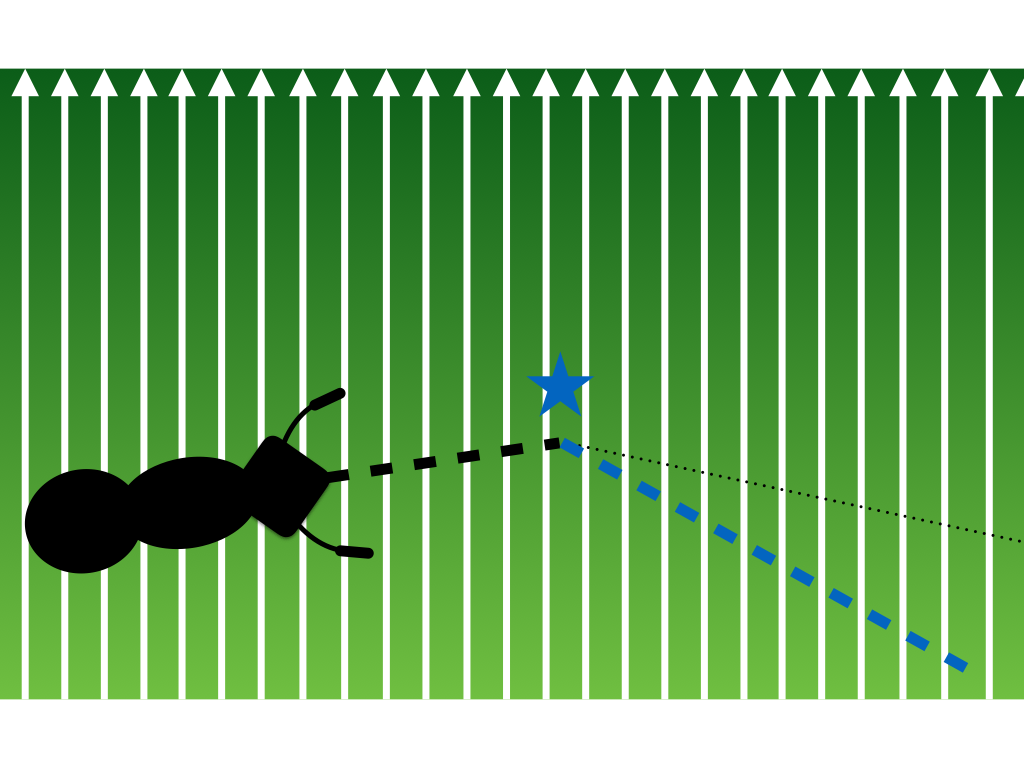
\includegraphics[width=0.6\textwidth]{images/model_components_cartoons_012}
\vspace{-2ex}
\caption{
\footnotesize{Illustration of adjustment accounting for ant behavior on uneven terrain}}
\end{figure}
\column{0.4\textwidth}
\begin{align*}
\bm{T}_{\operatorname{effective}} = \bm{T} / \beta \\
\beta =
\begin{cases}
      \text{forager role} & e^{c_1p} \\
      \text{returner role} & c_2
\end{cases} \\
s_{\operatorname{thresh}} = \bm{X} + c_3 \frac{|\vec{s} \cdot \vec{v}|}{\norm{\vec{v}}}
\end{align*}

\end{columns}
\begin{itemize}
  \item free path of ant ($s_{\operatorname{thresh}}$) increases if ant oriented with or against the gradient {\scriptsize\cite{khuong_how_2013}}
  \item ants preferentially re-orient themselves to align with or against a surface's topographical gradient {\scriptsize\cite{khuong_how_2013}}
	\item severity of random reorientation decreased when following pheromone trail and returning to nest
\end{itemize}
\end{frame}

% \begin{frame}{Events}
% \alert{behavioral effect of incline:}
% \begin{itemize}
% \end{itemize}
% \begin{columns}[T,onlytextwidth]
% \column{\textwidth}

% \begin{figure}
% \begin{minipage}[]{0.3\textwidth}
%     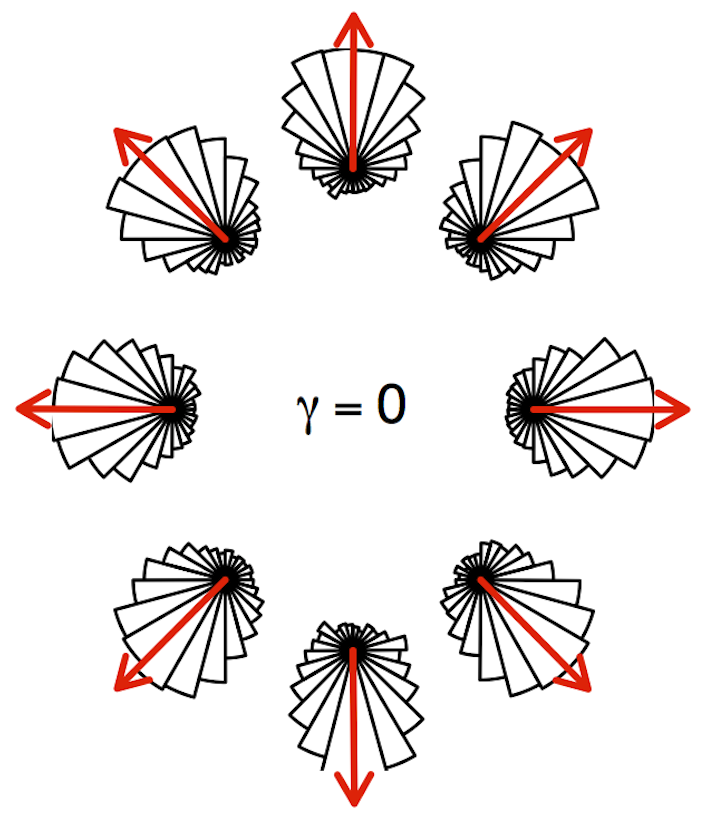
\includegraphics[width=\textwidth]{images/khuong_0}
% \end{minipage}%
% \begin{minipage}[]{0.05\textwidth}
% ~
% \end{minipage}%
% \begin{minipage}[]{0.3\textwidth}
%     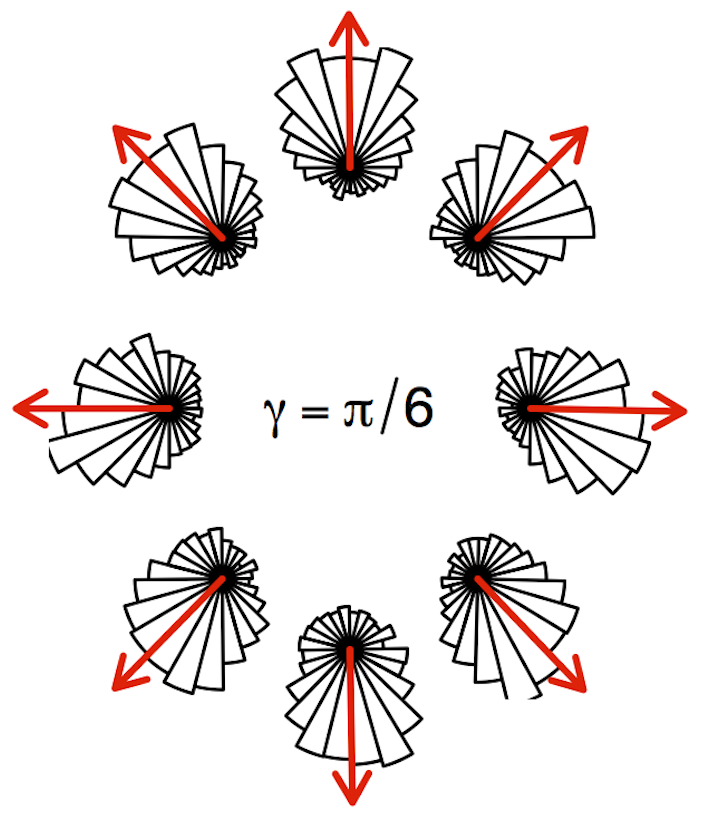
\includegraphics[width=\textwidth]{images/khuong_pi_div_6}
% \end{minipage}%
% \begin{minipage}[]{0.05\textwidth}
% ~
% \end{minipage}%
% \begin{minipage}[]{0.3\textwidth}
%     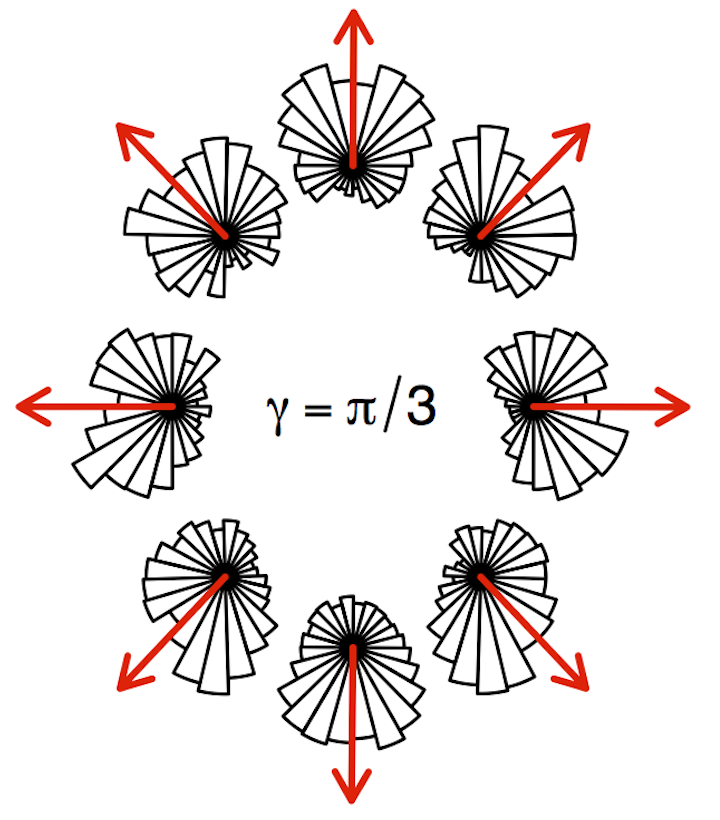
\includegraphics[width=\textwidth]{images/khuong_pi_div_3}
% \end{minipage}%
% \caption{Ant Reorientation on Inclined Surfaces \scriptsize{\cite{khuong_how_2013}}}
% \end{figure}
% \end{columns}

% \end{frame}

\end{subsection}


\begin{subsection}{Complete System}

\begin{frame}{Complete System}
\scriptsize
\centerline{
\begin{minipage}{\linewidth}
\begin{align*}
\frac{d}{dt}
\begin{pmatrix}
    \vec{x}_1 \\
    \vec{v}_1 \\
    s_1 \\
    \vdots \\
    p_1 \\
    \vdots
\end{pmatrix}
= \begin{pmatrix}
	\vec{v}_1 \\
    \alpha \hat{\vec{v}}_1 \Big[ \frac{c}{\norm{\vec{v}}} - a \norm{\vec{v}} + \frac{\norm{\vec{v}}^2 - b \vec{v} \cdot \nabla s}{\sqrt{\norm{\vec{v}}^2 + (\vec{v} \cdot \nabla s)^2}} \Big] + \beta_{\vec{x}} \frac{\vec{a} - \vec{x}_1}{\norm{\vec{a} - \vec{x}_1}} + \hat{\vec{v}}_{1\perp}(L_1 - R_1) + \gamma_{\vec{x}} \hat{\vec{v}}_{\perp} \Big( \hat{\vec{v}}_{\perp} \cdot \frac{\vec{a} - \vec{x}}{\norm{\vec{a} - \vec{x}}} \Big) \\
    \norm{\vec{v}_1} \\
    \vdots \\
    \kappa f(p_1, \vec{x}_1,\hdots,\vec{x}_n) + \lambda p_1 \\
    \vdots
\end{pmatrix}
\end{align*}
\end{minipage}
}
\normalsize
~\\
~\\
events:
\vspace{-2ex}
\begin{itemize}
\item out of bounds $\rightarrow$ reflect heading to ``bounce'' ant
\item $s > s_{\operatorname{thresh}}$ $\rightarrow$ $s = 0$, $s_{\operatorname{thresh}} = \bm{X} + c_3 \frac{|\vec{s} \cdot \vec{v}|}{\norm{\vec{v}}}$, random reorientation event with gradient alignment bias
\item close to food/nest $\rightarrow$ switch forager/returner role
\end{itemize}

\end{frame}

\begin{frame}{Animation}
	\begin{figure}
		\begin{center}
		\includemedia[width=\linewidth,height=0.6\textwidth, flashvars={scaleMode=zoom}]{}{http://www.youtube.com/v/YO6So6tgGVg?rel=0&amp;showinfo=0}
		\end{center}
		\caption{\href{http://www.youtube.com/v/YO6So6tgGVg?rel=0&amp;showinfo=0}{Animation of numerically-approximated solution}}
	\end{figure}
\end{frame}


\end{subsection}

\begin{section}{Results}


\begin{frame}{Results (preliminary): Path Shape}
\begin{figure}
\begin{columns}[T,onlytextwidth]
\column{0.33\textwidth}
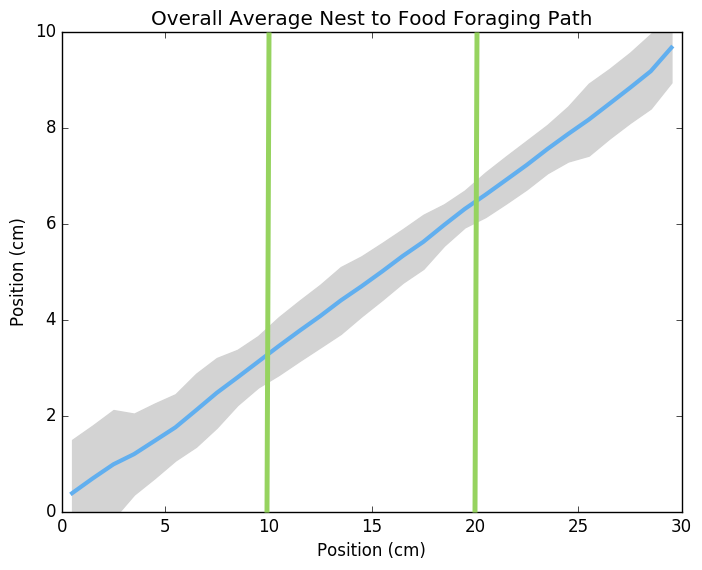
\includegraphics[width=\textwidth]{results/corner-to-corner-average_path_negpidiv3.png}
\column{0.005\textwidth}
\column{0.33\textwidth}
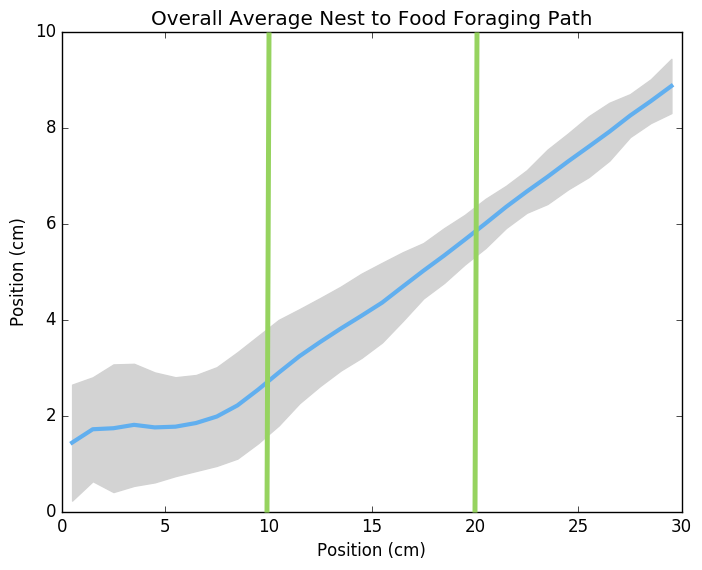
\includegraphics[width=\textwidth]{results/corner-to-corner-average_path_0.png}
\column{0.005\textwidth}
\column{0.33\textwidth}
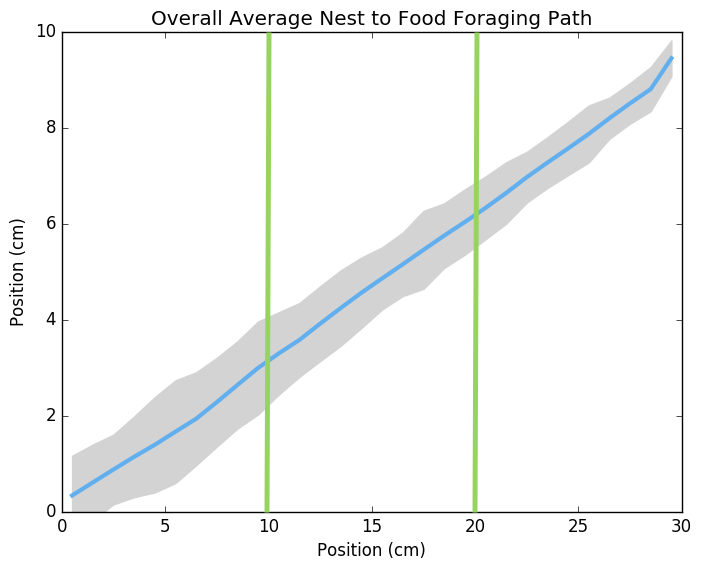
\includegraphics[width=\textwidth]{results/corner-to-corner-average_path_pidiv3.png}
\end{columns}
\caption{Comparison of overall average nest to food foraging path for, left to right, $-\pi/3$, $0$, and $\pi/3$ radian inclines.}
\end{figure}
\end{frame}


\begin{frame}{Results (preliminary): Path Length}
\begin{figure}
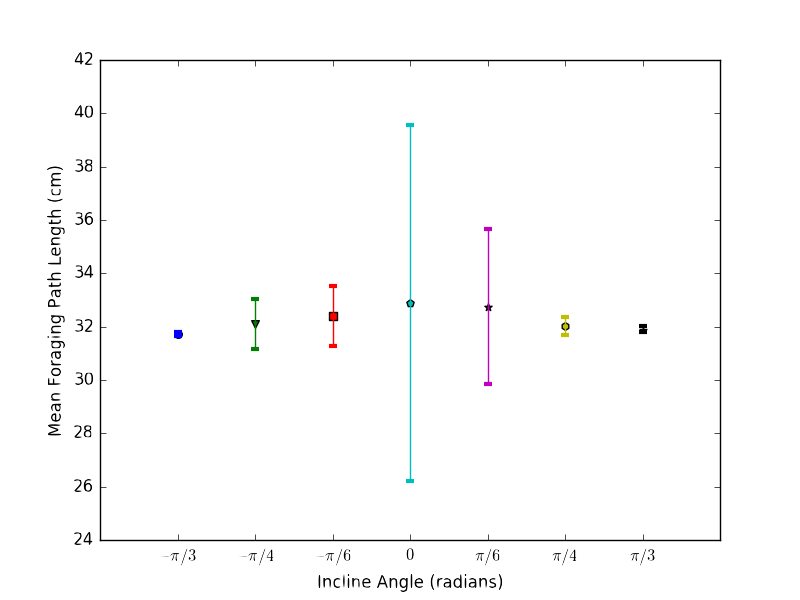
\includegraphics[width=0.8\textwidth]{results/corner-to-cornermeanforagingpathlength.png}
\caption{Comparison of path lengths over incline angles for corner-to-corner trials}
\end{figure}
\end{frame}


\begin{frame}{Next Steps}
\begin{columns}[T,onlytextwidth]
\column{0.5\textwidth}
\begin{itemize}
\item Refine model
	\begin{itemize}
		\item variable pheromone deposition rate
	\end{itemize}
\item Perform further sensitivity analyses
	\begin{itemize}
		\item pheromone grid granularity
        \item pheromone sensitivity radius of ant
        \item behavioral weighting
	\end{itemize}
%\item Perform replicate simulations
%\item Explore further combinations of experimental conditions
% \item More sophisticated analysis of ant paths (Splines?)
\item \textbf{Compare model predictions with empirical results}
\end{itemize}
\column{0.1\textwidth}
\column{0.4\textwidth}
\begin{figure}
        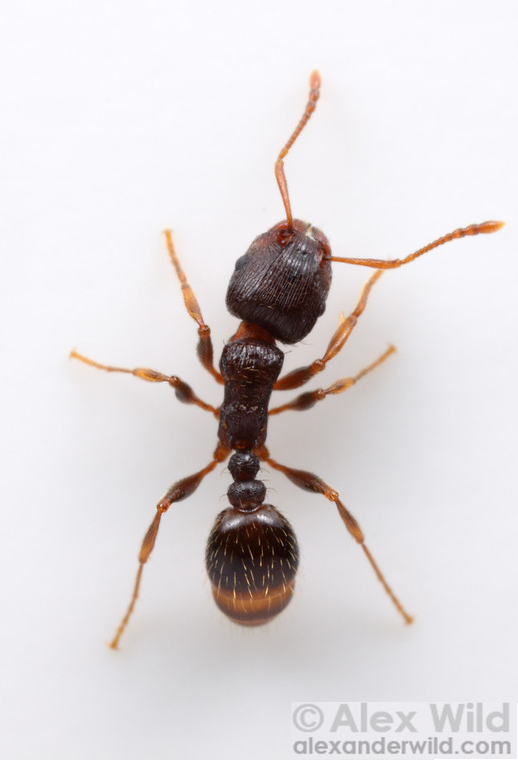
\includegraphics[width=\textwidth]{images/spE2-XL}
        \caption{\textit{Tetramorium caespitum} \scriptsize{\cite{spE2-XL.jpg_????}}}
\end{figure}
\end{columns}
\end{frame}


% \begin{frame}{Results (preliminary): Summary}
% \begin{itemize}
% 	\item as expected, foraging trips take longer over steeper incline and decline
% 	\begin{itemize}
% 		\item also taking longer over uphill versus downhill inclines
% 	\end{itemize}
% 	\vspace{1em}

% 	\item the foraging path is generally more stable with steep incline or decline
% 	\begin{itemize}
% 		%\item path is smoother
% 		\item ants are less likely to get lost/stuck
% 		\item this effect is less pronounced in the center-to-center arena
% 	\end{itemize}
% 	\vspace{1em}

% 	\item the foraging path becomes more direct with steeper incline or decline
% 	\vspace{-1em}
% 	\begin{itemize}
% 		\item even though the direct path is not aligned with the incline in the corner-to-corner arena
% 		\item this effect is less pronounced in the center-to-center arena
% 	\end{itemize}
% \end{itemize}
% \end{frame}

\end{section}

\begin{frame}{Acknowledgements}
\begin{itemize}
\item Dr. Garnier and Dr. Graham for their excellent mentorship
\item New Jersey Institute of Technology and The Ohio State University
\item Mathematical Biosciences Institute (MBI) REU program
\item My advisors and mentors at the University of Puget Sound
\item This material is based upon work supported by the National Science Foundation under Grant No. 1461163
\end{itemize}
\begin{columns}[T,onlytextwidth]
\column{\textwidth}
\begin{minipage}[]{0.0125\textwidth}
~
\end{minipage}%
\begin{minipage}[]{0.225\textwidth}
    
\includegraphics[width=\textwidth]{images/mbiwtext}
\end{minipage}%
\begin{minipage}[]{0.025\textwidth}
~
\end{minipage}%
\begin{minipage}[]{0.225\textwidth}
    
\includegraphics[width = \textwidth]{images/Logo_of_New_Jersey_Institute_of_Technology}
\end{minipage}%
\begin{minipage}[]{0.025\textwidth}
~
\end{minipage}%
\begin{minipage}[]{0.225\textwidth}
    
\includegraphics[width = \textwidth]{images/OSU_Stacked_ScarletBlack}
\end{minipage}%
\begin{minipage}[]{0.025\textwidth}
~
\end{minipage}%
\begin{minipage}[]{0.225\textwidth}
    
\includegraphics[width = \textwidth]{images/UofPS_stacked_maroonRGB_PNG}
\end{minipage}%
\begin{minipage}[]{0.0125\textwidth}
~
\end{minipage}%
\end{columns}
\end{frame}

\begin{frame}[standout]
  Questions?
\end{frame}

\appendix

\begin{frame}[allowframebreaks]{References}
  \setbeamertemplate{bibliography item}{\insertbiblabel}
  %\nocite{*} % Insert publications even if they are not cited in the poster
  \bibliographystyle{apalike}
  \bibliography{main.bib}
\end{frame}


\begin{frame}{Background}
	\begin{figure}
		\begin{center}
		\includemedia[width=\linewidth,height=0.6\textwidth, flashvars={scaleMode=zoom}]{}{http://www.youtube.com/v/QeSErcTOLbY?rel=0&amp;showinfo=0}
		\end{center}
		\caption{\href{http://www.youtube.com/v/QeSErcTOLbY?rel=0&amp;showinfo=0}{Video clip demonstrating route selection by foraging ants}}
	\end{figure}
\end{frame}

\begin{frame}{Motivation}
\vspace{0.5em}

\begin{figure}
\begin{columns}%
        \begin{column}{0.75\textwidth}%
            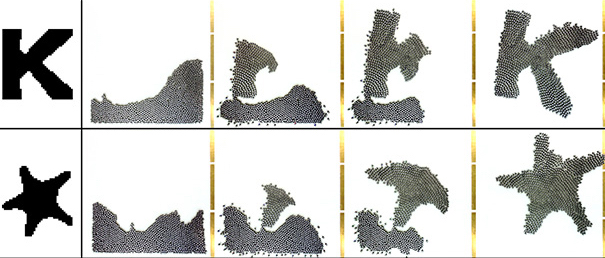
\includegraphics[width=\textwidth,right]{images/Kilobots31}
        \end{column}%
        \begin{column}{0.25\textwidth}%
            \caption{Kilobots in action \scriptsize{\cite{mike_rubenstein_kilobots31_2014}}}
        \end{column}%
    \end{columns}
\end{figure}

\vspace{1.5em}
\begin{figure}
\begin{columns}%
        \begin{column}{0.75\textwidth}%
            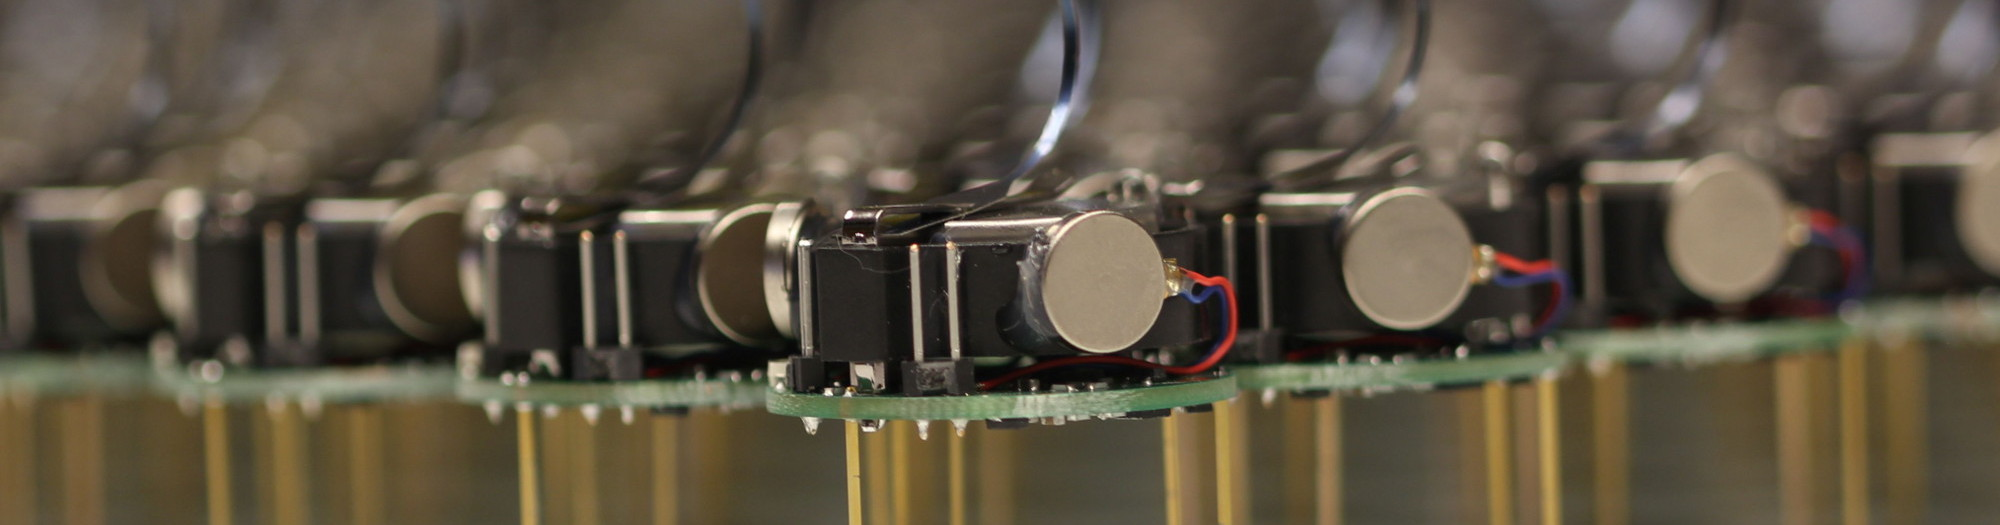
\includegraphics[width=\textwidth,right]{images/kilobots}
        \end{column}%
        \begin{column}{0.25\textwidth}%
            \caption{Kilobots, a common swarm robotics platform \scriptsize{\cite{ssr_lab_harvard_university_swarm2.jpg_????}}}
        \end{column}%
    \end{columns}
\end{figure}

\end{frame}

\begin{frame}{Background}
	\begin{figure}
		\begin{center}
		\includemedia[width=\linewidth,height=0.6\textwidth, flashvars={scaleMode=zoom}]{}{http://www.youtube.com/v/c7kiPri9ZFo?rel=0&amp;showinfo=0}
		\end{center}
		\caption{\href{http://www.youtube.com/v/c7kiPri9ZFo?rel=0&amp;showinfo=0}{Video clip of pheromone deposit and response by foraging ants}}
	\end{figure}
\end{frame}

\begin{frame}{System of Ordinary Differential Equations: Single Ant}

\begin{columns}[T,onlytextwidth]
    \column{0.45\textwidth}
     \alert{effect of pheromone:}
\begin{itemize}
	%\item ant integrates pheromone concentration over ``L'' and ``R'' quarter-circular regions
    \item ant accelerates perpendicular to its orientation
    \item magnitude of acceleration is proportional to the difference in concentration of pheromone over the ``L'' and ``R'' regions
\end{itemize}

	\column{0.1\textwidth}
    \column{0.45\textwidth}

      \begin{align*}
\frac{d}{dt} \begin{pmatrix}\vec{x}\\\vec{v}\end{pmatrix} = \begin{pmatrix}\hdots\\ \hat{\vec{v}}_{\perp}(L - R)\end{pmatrix}
\end{align*}
 \begin{figure}
    	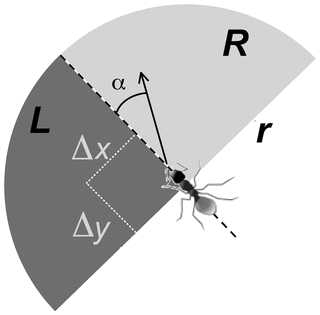
\includegraphics[height=3cm]{images/l_r_regions}
        \caption{Regions of ant sensitivity to pheromone \scriptsize{\cite{perna_individual_2012}}}
    \end{figure}

  \end{columns}
\end{frame}

\begin{frame}{Results (preliminary): Quickest Center-to-Center Path}
\begin{figure}
\begin{columns}[T,onlytextwidth]
\column{0.5\textwidth}
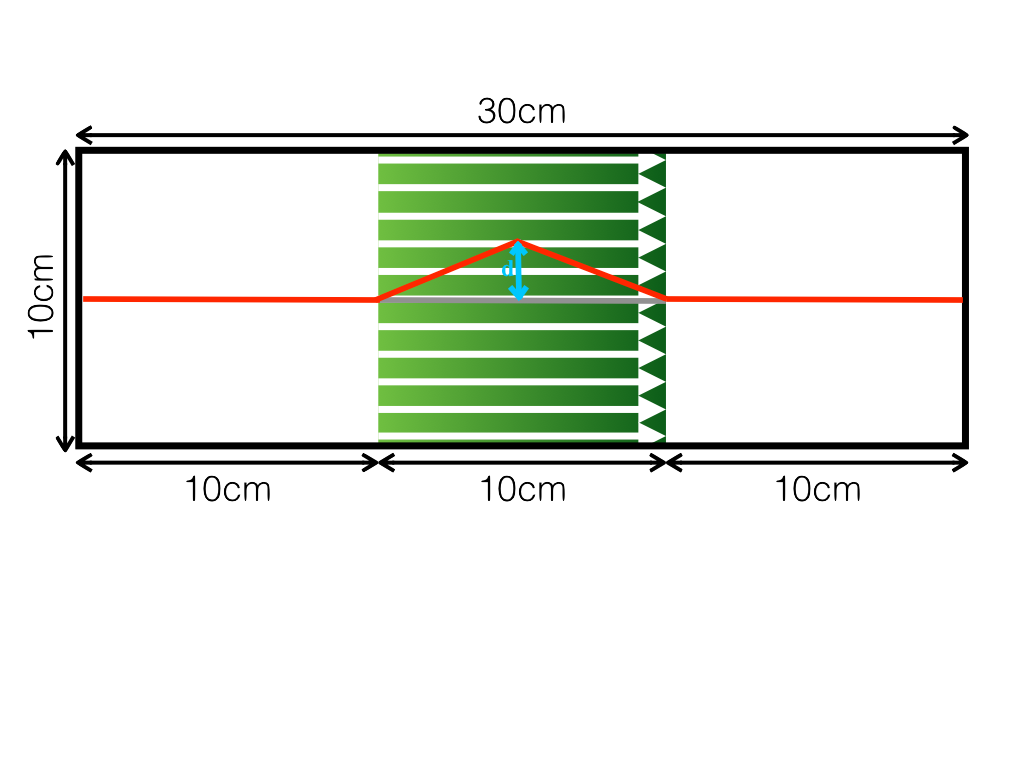
\includegraphics[width=\textwidth]{images/optimal_cen_cen_schematic}
\column{0.5\textwidth}
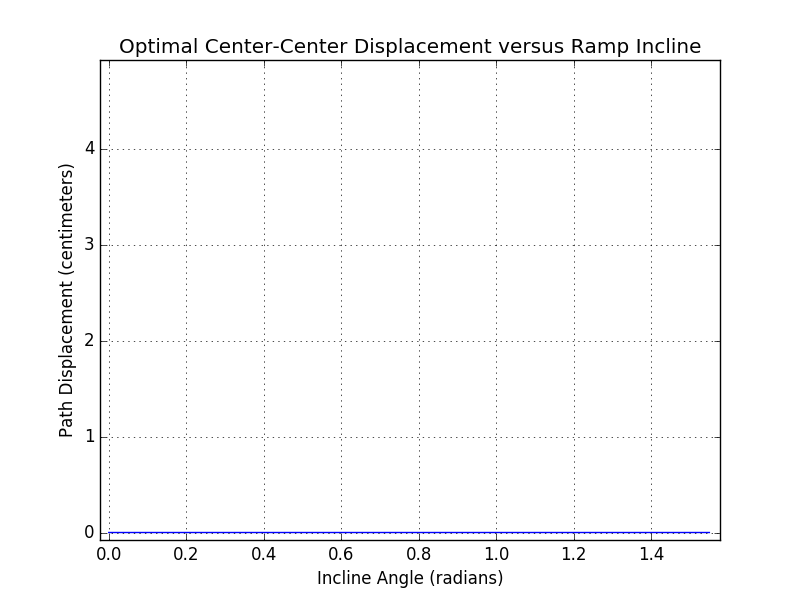
\includegraphics[width=\textwidth]{images/optimal_center_center}
\end{columns}
\caption{Plot of optimal displacement for quickest center-to-center path with schematic showing displacement.}
\end{figure}
\end{frame}

\begin{frame}{Results (preliminary): Quickest Corner-to-Corner Path}
\begin{figure}
\begin{columns}[T,onlytextwidth]
\column{0.5\textwidth}
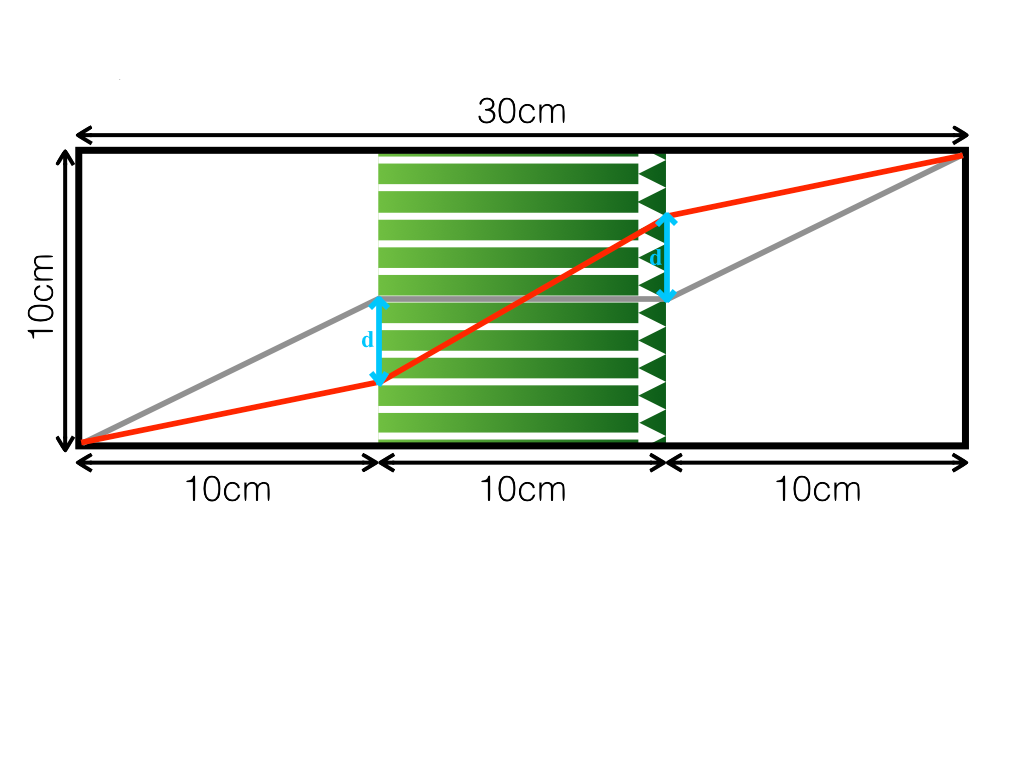
\includegraphics[width=\textwidth]{images/optimal_cor_cor_schematic}
\column{0.5\textwidth}
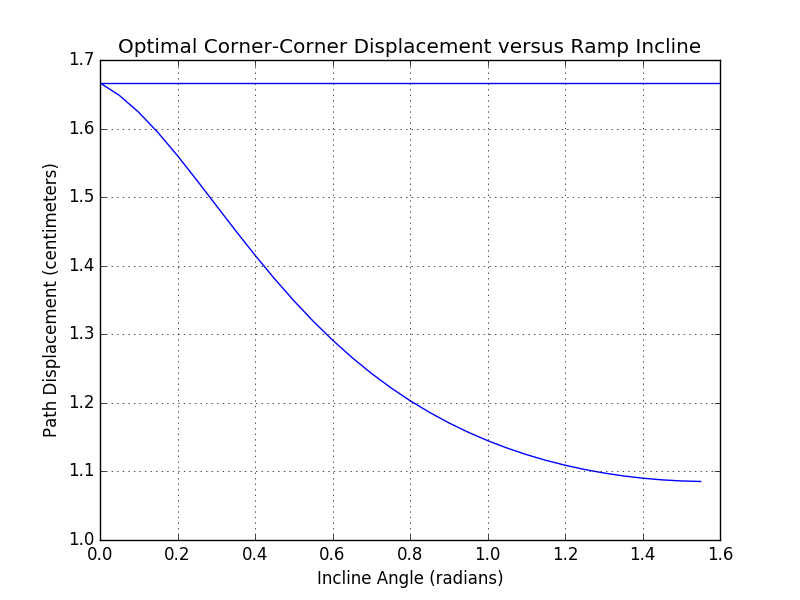
\includegraphics[width=\textwidth]{images/optimal_corner_corner}
\end{columns}
\caption{Plot of optimal displacement for quickest corner-to-corner path with schematic showing displacement.}
\end{figure}
\end{frame}

\begin{frame}{Results (preliminary): Path Shape}
\begin{figure}
\begin{columns}[T,onlytextwidth]
\column{0.33\textwidth}
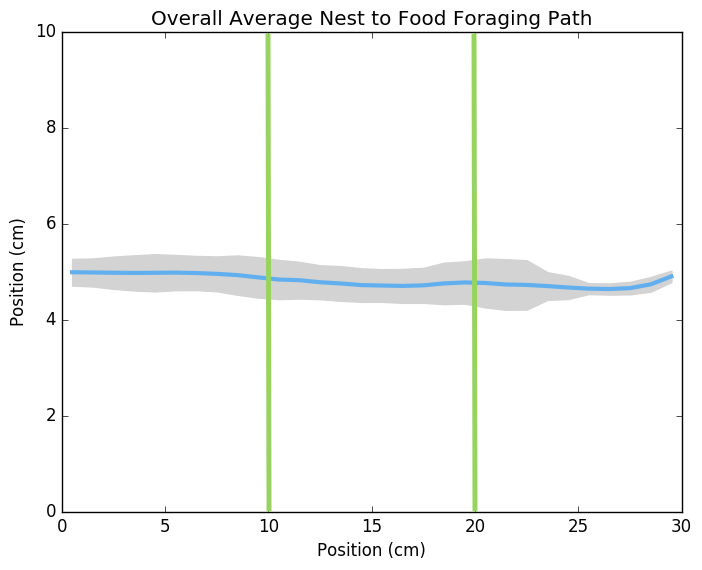
\includegraphics[width=\textwidth]{results/center-to-center-average_path_negpidiv3.png}
\column{0.005\textwidth}
\column{0.33\textwidth}
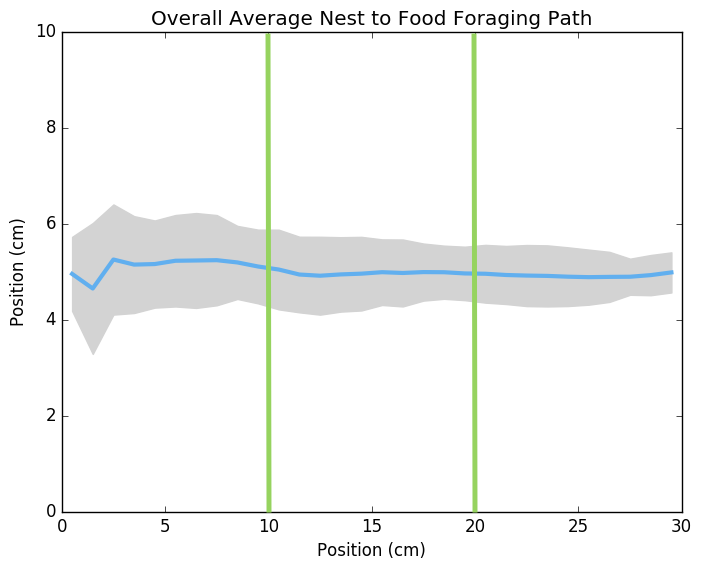
\includegraphics[width=\textwidth]{results/center-to-center-average_path_0.png}
\column{0.005\textwidth}
\column{0.33\textwidth}
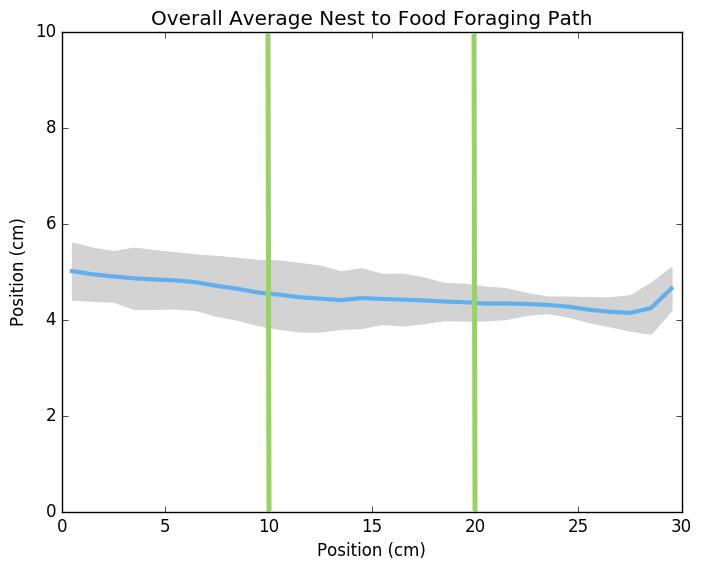
\includegraphics[width=\textwidth]{results/center-to-center-average_path_pidiv3.png}
\end{columns}
\caption{Comparison of overall average nest to food foraging path for, left to right, $-\pi/3$, $0$, and $\pi/3$ radian inclines.}
\end{figure}
\end{frame}

\begin{frame}{Results (preliminary): Path Length}
\begin{figure}
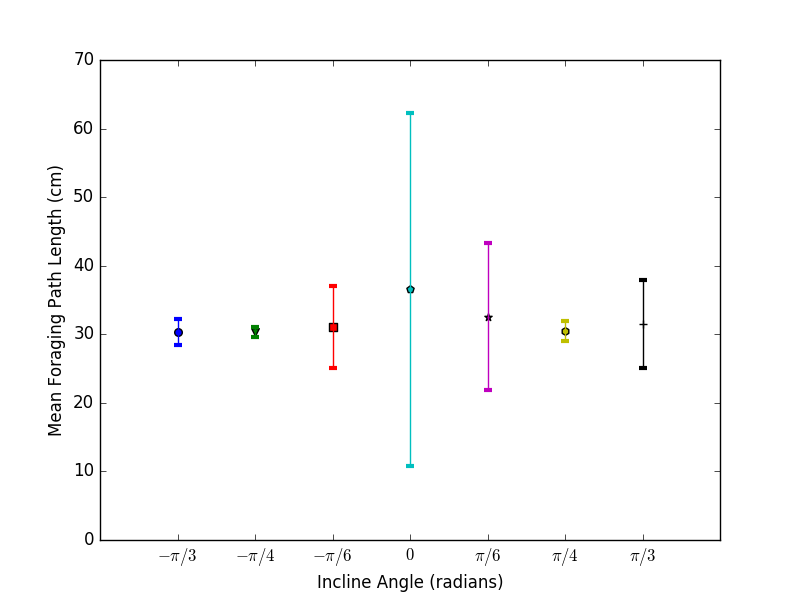
\includegraphics[width=0.8\textwidth]{results/center-to-centermeanforagingpathlength.png}
\caption{Comparison of path lengths over incline angles for center-to-center trials}
\end{figure}
\end{frame}

\begin{frame}{Results (preliminary): Path Smoothness}
\begin{figure}
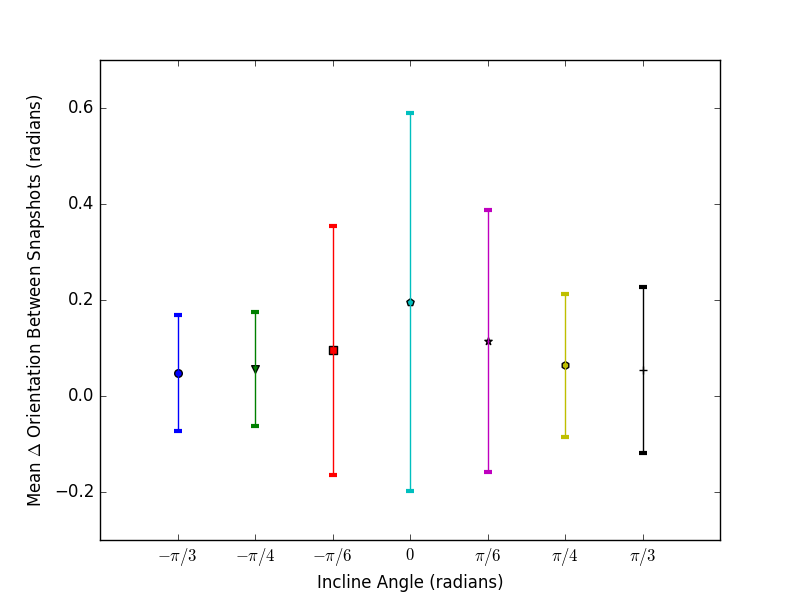
\includegraphics[width=0.8\textwidth]{results/center-to-center_meandeltaorientationbetweensnapshots.png}
\caption{Comparison of changes in heading between shapshots over incline angles for center-to-center trials}
\end{figure}
\end{frame}

\begin{frame}{Results (preliminary): Trip Duration}
\begin{figure}
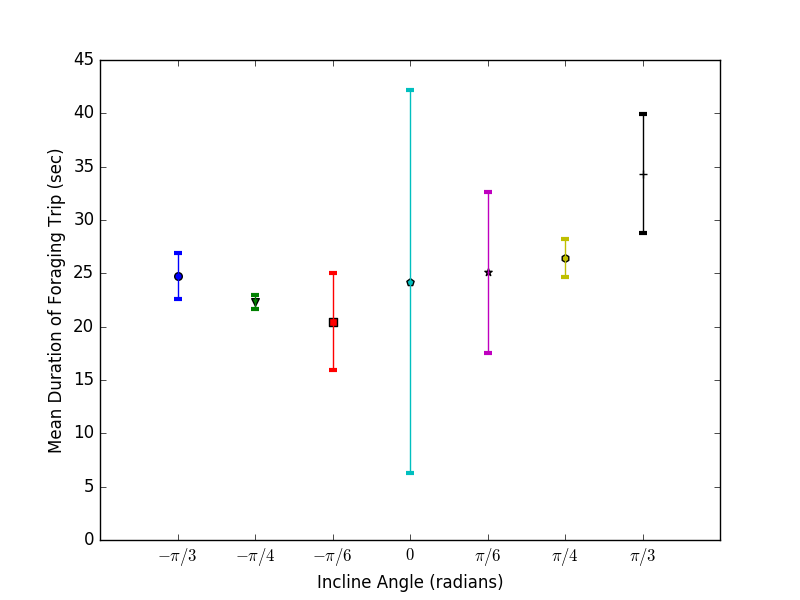
\includegraphics[width=0.8\textwidth]{results/center-to-centermeandurationofforagingtrip.png}
\caption{Comparison of trip durations over incline angles for center-to-center trials}
\end{figure}
\end{frame}

\begin{frame}{Results (preliminary): Orientation Relative to Gradient}
\begin{figure}
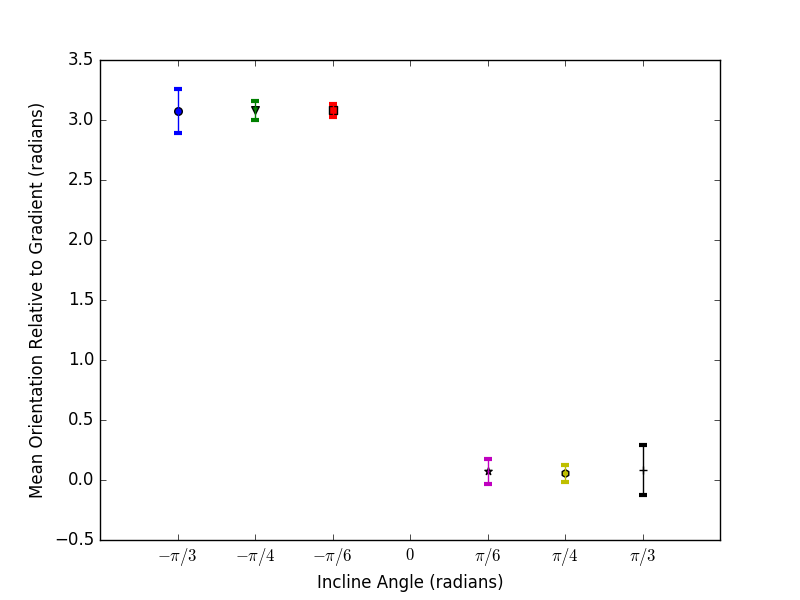
\includegraphics[width=0.8\textwidth]{results/center-to-centermeanorientationrelativetogradient.png}
\caption{Comparison of orientation relative to gradient over incline angles for center-to-center evaporation rates; the straight path is oriented at 0/3.14 radians}
\end{figure}
\end{frame}

\begin{frame}{System of Ordinary Differential Equations: Single Ant}

    	\begin{align*}
			\frac{d}{dt} \begin{pmatrix}\vec{x}\\\vec{v}\end{pmatrix} = \begin{pmatrix}\vec{v}\\ \alpha \hat{\vec{v}}(\xi^2 - \norm{\vec{v}}^2)\end{pmatrix}
		\end{align*}

\alert{self-propulsion: \cite{ryan_model_2016}}
\begin{itemize}
	\item ant accelerates in the direction of its movement if $\norm{\vec{v}}  \xi$
    \item ant accelerates against the direction of its movement if $\norm{\vec{v}} < \xi$
    \item``pushes'' ant towards a fixed speed
    \item $\alpha$ is a constant that governs the magnitude of this effect
\end{itemize}
\end{frame}

\begin{frame}{System of Ordinary Differential Equations: Single Ant}
\begin{align*}
\frac{d}{dt} \begin{pmatrix}\vec{x}\\\vec{v}\end{pmatrix} = \begin{pmatrix}\hdots \\ \beta_{\vec{x}} \frac{\vec{a} - \vec{x}}{\norm{\vec{a} - \vec{x}}} \end{pmatrix}
\end{align*}
\alert{attraction to food/nest:}
\begin{itemize}
	\item ant experiences nest attraction if it is in the returner role
    \item ant experiences food attraction if it is in the forager role
	\item ant accelerates in the direction of the attractor
    \item if multiple attractors are present,
    \begin{itemize}
		\item ant is attracted to nearest food item
        \item ant is attracted to midpoint of nest items
    \end{itemize}
    \item $\beta_{\vec{x}}$ governs the strength of attraction
    \begin{itemize}
    	\item constant for nest attraction
        \item for food attraction, decays exponentially with distance from food
    \end{itemize}
\end{itemize}
\end{frame}

\begin{frame}{System of Ordinary Differential Equations: Single Ant}
\begin{align*}
\frac{d}{dt} \begin{pmatrix}\vec{x}\\\vec{v}\end{pmatrix} = \begin{pmatrix}
\hdots \\
\gamma_{\vec{x}} \hat{\vec{v}}_{\perp} \Big( \hat{\vec{v}}_{\perp} \cdot \frac{\vec{a} - \vec{x}}{\norm{\vec{a} - \vec{x}}} \Big)
\end{pmatrix}  \\
\beta = c_1e^{-c_2\norm{\vec{a} - \vec{x}}}
\end{align*}
\alert{near nest attraction:}
\begin{itemize}
	\item ant experiences attraction with magnitude increasing exponentially with proximity to nest
    \item acceleration is projected onto vector perpendicular to orientation of ant
	\item ensures that ant goes directly to nest if ant is nearby the nest
\end{itemize}
\end{frame}

\begin{frame}{System of Ordinary Differential Equations: Pheromone Deposit}
\begin{align*}
\frac{d}{dt} p = \kappa f(p,s\vec{x}_1,\hdots,\vec{x}_n)
\end{align*}
\alert{pheromone deposit:}
\begin{itemize}
	\item the rate of pheromone deposit is proportional to total speed of ants located at a tile
    \item (ants only deposit pheromone when they move)
    \item let $f(p, \vec{x}_1,\hdots,\vec{x}_n)$ represent a sum of the speeds of of ants associated with the pheromone point $p$
    \item $\kappa$ is a constant governing the magnitude of pheromone deposit
\end{itemize}
\end{frame}

\begin{frame}{Events}
\begin{columns}[T,onlytextwidth]
\column{0.70\textwidth}
\small{
\begin{align*}
t =
\begin{cases}
      0 & \bm{U}_1 < \gamma\frac{b_1 - a_1(\cos^2(\phi)-\sin^2(\phi))[c_1 - \hat{\vec{v}} \cdot \hat{\nabla S}]}{\pi/3} \\
      1 & \text{otherwise}
   \end{cases}
\end{align*}
\begin{align*}
s =
\begin{cases}
      -1 & \bm{U}_2 < \frac{\pi -2 d_2 \cos(\phi) [a_2-2 b_2 \sin(\phi)]}{2 \pi } \\
      1 & \text{otherwise}
   \end{cases}
\end{align*}
}
\column{0.05\textwidth}
\column{0.25\textwidth}
\begin{align*}
\theta_{\operatorname{new}} = \theta_{\operatorname{old}} + \bm{T},\\
\bm{T} \sim \mathcal{N}(\pi/6 \times g,\sigma^2), \\
g = s \times t, \\
\bm{U}_1, \bm{U}_2 \sim \operatorname{unif}(0,1)
\end{align*}
\end{columns}
\alert{random reorientation events on an incline:}
\begin{itemize}
	\item ant reorientation is biased by $-\pi/6$, $0$, or $\pi/6$ radians
	 \item random choices made
     \begin{itemize}
     	\item whether to turn or proceed straight
     	\item if turning, whether to turn left or right
     \end{itemize}
     \item probabilities of these choices determined by
     \begin{itemize}
     	\item $\phi$, ant orientation relative to gradient
        \item $\gamma$, angle of inclination
     \end{itemize}
\end{itemize}
\end{frame}

\begin{frame}{Events}
\alert{random reorientation events on an incline:}
\begin{itemize}
     \item parameters were fit using Matlab's \texttt{lsqcurvefit} and  \scriptsize{\cite{khuong_how_2013}}
\end{itemize}
\begin{figure}
\begin{columns}[T,onlytextwidth]
\column{\textwidth}
\begin{minipage}[]{0.05\textwidth}
~
\end{minipage}%
\begin{minipage}[]{0.315\textwidth}
    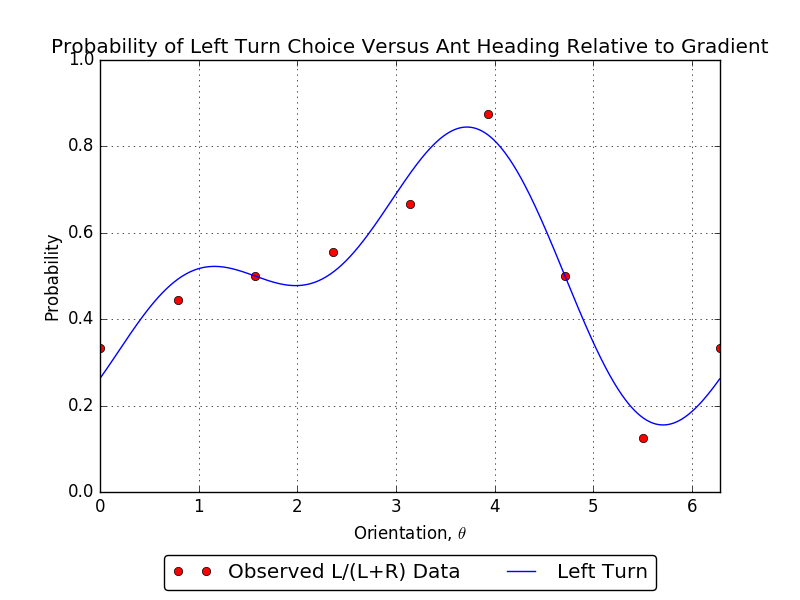
\includegraphics[width=\textwidth]{images/l_choice} \\
    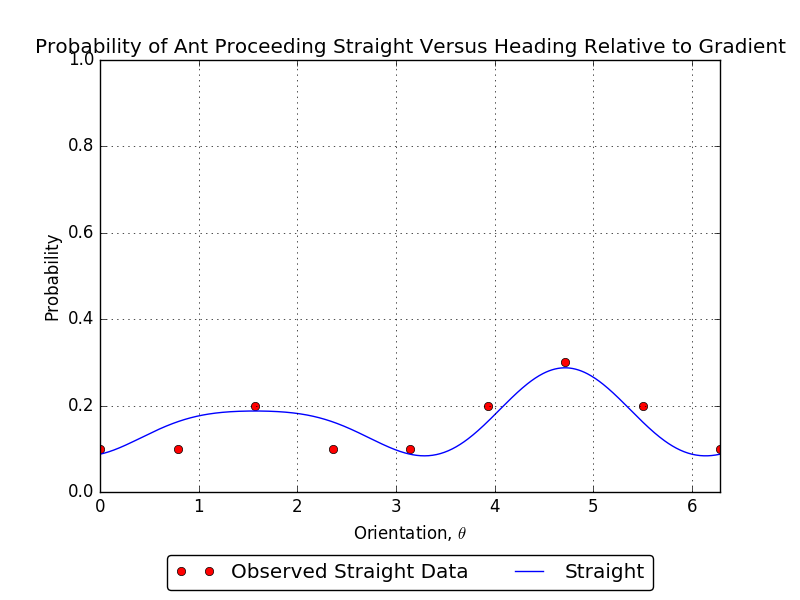
\includegraphics[width = \textwidth]{images/s_choice}
\end{minipage}%
\begin{minipage}[]{0.045\textwidth}
~
\end{minipage}%
\begin{minipage}[]{0.54\textwidth}
    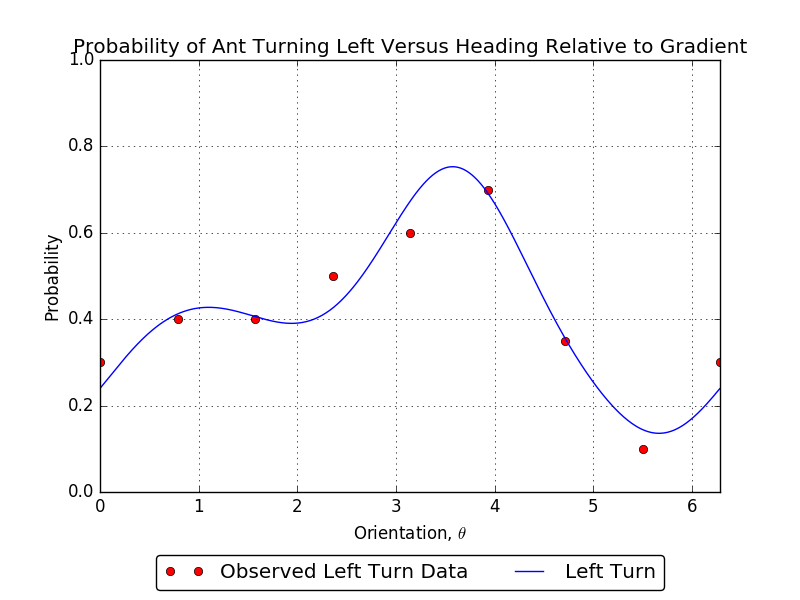
\includegraphics[width = \textwidth]{images/l_result}
\end{minipage}%
\begin{minipage}[]{0.05\textwidth}
~
\end{minipage}%
\end{columns}
\caption{Ant reorientation behavior on an incline ($\gamma = \pi/3$), observed in \cite{khuong_how_2013} versus approximated}
\end{figure}
\end{frame}


\begin{frame}{Numerical Approximation}

\begin{itemize}
	\item deriving an analytic solution is intractable
    \item take a series of small time steps, using each time point to approximate the next
    \item Matlab provides a set of ODE solvers that implement sophisticated algorithms for generating numerical solutions to systems of differential equations
    \item \texttt{ode113} was selected to perform simulations
\end{itemize}
\end{frame}

\begin{frame}{Sensitivity Analysis: Pheromone Evaporation Rate}
	\begin{figure}
	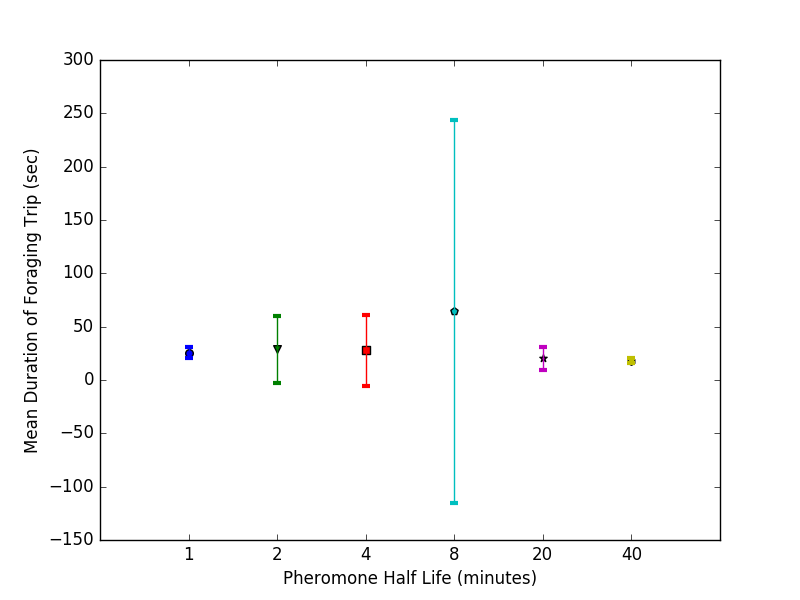
\includegraphics[width=0.8\textwidth]{results/center-to-center-sensitivityanalysis-duration.png}
	\caption{Comparison of durations over pheromone evaporation half lives for center-to-center trials.}
	\end{figure}
\end{frame}

\begin{frame}{Sensitivity Analysis: Pheromone Evaporation Rate}
	\begin{figure}
	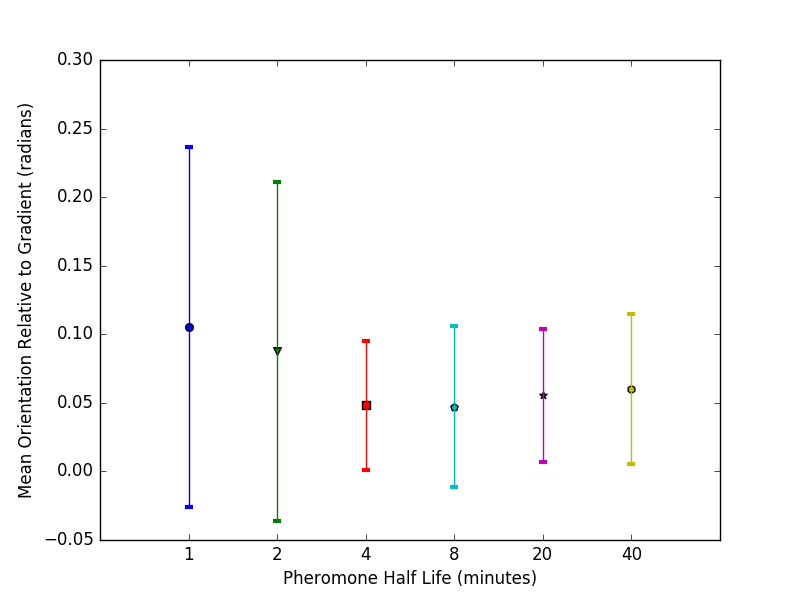
\includegraphics[width=0.8\textwidth]{results/center-to-center-sensitivityanalysis-meanorientation.png}
	\caption{Comparison of orientations relative to gradient over pheromone evaporation half lives for center-to-center trials.}
	\end{figure}
\end{frame}

\begin{frame}{Sensitivity Analysis: Pheromone Evaporation Rate}
	\begin{figure}
	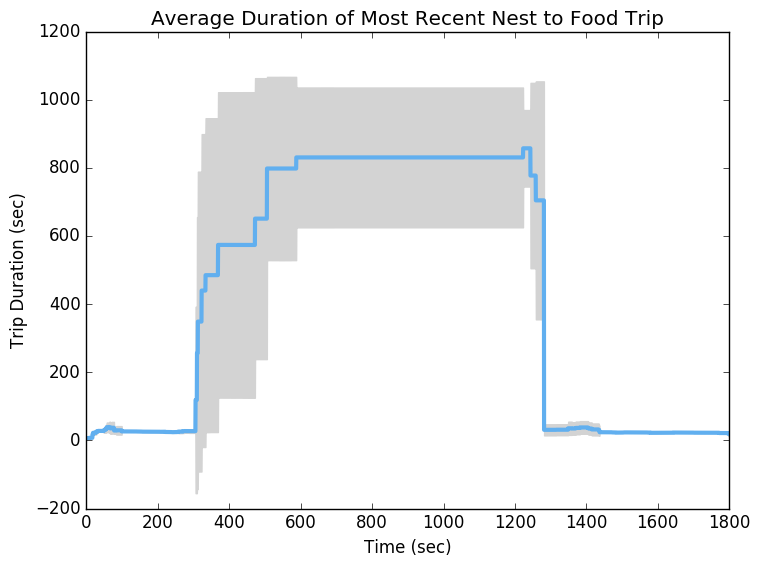
\includegraphics[width=0.8\textwidth]{results/center-to-center-average-trip-duration-8xpheromone.png}
	\caption{Average trip duration over the course of a 30 minute simulation in a center-to-center arena with 8 minute pheromone half life.}
	\end{figure}
\end{frame}

\begin{frame}{Results (preliminary): Path Shape}
\begin{figure}
	\begin{center}
	\includemedia[width=\linewidth,height=0.6\textwidth, flashvars={scaleMode=zoom}]{}{http://www.youtube.com/v/QeSErcTOLbY?rel=0&amp;showinfo=0}
	\end{center}
	\caption{\href{http://www.youtube.com/v/QeSErcTOLbY?rel=0&amp;showinfo=0}{Visualization of path as simulation progresses}}
\end{figure}
\end{frame}

\begin{frame}{Results (preliminary): Path Smoothness}
\begin{figure}
\includegraphics[width=0.8\textwidth]{results/corner-to-corner_meandeltaorientationbetweensnapshots.png}
\caption{Comparison of changes in heading between shapshots over incline angles for corner-to-corner trials}
\end{figure}
\end{frame}

\begin{frame}{Results (preliminary): Orientation Relative to Gradient}
\begin{figure}
\includegraphics[width=0.8\textwidth]{results/corner-to-cornermeanorientationrelativetogradient.png}
\caption{Comparison of orientation relative to gradient over incline angles for corner-to-corner trials; the straight path is oriented at 2.819/0.321 radians}
\end{figure}
\end{frame}

\begin{frame}{Self 
Propulsion on Uneven Terrain}

\begin{align*}
\frac{d}{dt} \begin{pmatrix}\vec{x}\\\vec{v}\end{pmatrix} = \begin{pmatrix}\vec{v}\\ \hat{\vec{v}} \Big[ \frac{c}{\norm{\vec{v}}} - a \norm{\vec{v}} + \frac{\norm{\vec{v}}^2 - b \vec{v} \cdot \nabla s}{\sqrt{\norm{\vec{v}}^2 + (\vec{v} \cdot \nabla s)^2}} \Big] \end{pmatrix}
\end{align*}

\begin{columns}[T,onlytextwidth]

\column{0.45\textwidth}
\small{
\begin{itemize}
    \item ants choose walking speed to expend constant power {\scriptsize\cite{holt_locomotion_2012}}
    \item gravity opposes uphill movement, aids downhill movement
    \item severe incline/decline decreases overall efficiency of ant movement
    % \item $a$, $b$, $p$, constants governing this effect, were fitted using Matlab's \texttt{lsqcurvefit}
\end{itemize}
}
\column{0.1\textwidth}
\column{0.45\textwidth}
 \begin{figure}
    	\includegraphics[width=\textwidth]{images/const_power_velocity}
        \caption{Ant velocity under constant power on inclined terrain}
    \end{figure}
\end{columns}
\end{frame}

\begin{frame}{Experimental Design}

   \begin{figure}
    	\includegraphics[width=0.8\textwidth]{images/model_components_cartoons_010}
				\vspace{-8ex}
				\caption{Nest and food placement scheme}
    \end{figure}
\end{frame}

\begin{frame}{Results (preliminary): Trip Duration}
\begin{figure}
\includegraphics[width=0.8\textwidth]{results/corner-to-cornermeandurationofforagingtrip.png}
\caption{Comparison of trip durations over incline angles for corner-to-corner trials}
\end{figure}
\end{frame}

\end{document}
